\documentclass[]{article}
\usepackage{lmodern}
\usepackage{amssymb,amsmath}
\usepackage{ifxetex,ifluatex}
\usepackage{fixltx2e} % provides \textsubscript
\ifnum 0\ifxetex 1\fi\ifluatex 1\fi=0 % if pdftex
  \usepackage[T1]{fontenc}
  \usepackage[utf8]{inputenc}
\else % if luatex or xelatex
  \ifxetex
    \usepackage{mathspec}
  \else
    \usepackage{fontspec}
  \fi
  \defaultfontfeatures{Ligatures=TeX,Scale=MatchLowercase}
  \newcommand{\euro}{€}
\fi
% use upquote if available, for straight quotes in verbatim environments
\IfFileExists{upquote.sty}{\usepackage{upquote}}{}
% use microtype if available
\IfFileExists{microtype.sty}{%
\usepackage{microtype}
\UseMicrotypeSet[protrusion]{basicmath} % disable protrusion for tt fonts
}{}
\usepackage[margin=2.54cm]{geometry}
\usepackage{hyperref}
\PassOptionsToPackage{usenames,dvipsnames}{color} % color is loaded by hyperref
\hypersetup{unicode=true,
            pdftitle={Assignment: Temporal Diversity},
            pdfauthor={Katie Beidler; Z620: Quantitative Biodiversity, Indiana University},
            pdfborder={0 0 0},
            breaklinks=true}
\urlstyle{same}  % don't use monospace font for urls
\usepackage{color}
\usepackage{fancyvrb}
\newcommand{\VerbBar}{|}
\newcommand{\VERB}{\Verb[commandchars=\\\{\}]}
\DefineVerbatimEnvironment{Highlighting}{Verbatim}{commandchars=\\\{\}}
% Add ',fontsize=\small' for more characters per line
\usepackage{framed}
\definecolor{shadecolor}{RGB}{248,248,248}
\newenvironment{Shaded}{\begin{snugshade}}{\end{snugshade}}
\newcommand{\KeywordTok}[1]{\textcolor[rgb]{0.13,0.29,0.53}{\textbf{{#1}}}}
\newcommand{\DataTypeTok}[1]{\textcolor[rgb]{0.13,0.29,0.53}{{#1}}}
\newcommand{\DecValTok}[1]{\textcolor[rgb]{0.00,0.00,0.81}{{#1}}}
\newcommand{\BaseNTok}[1]{\textcolor[rgb]{0.00,0.00,0.81}{{#1}}}
\newcommand{\FloatTok}[1]{\textcolor[rgb]{0.00,0.00,0.81}{{#1}}}
\newcommand{\ConstantTok}[1]{\textcolor[rgb]{0.00,0.00,0.00}{{#1}}}
\newcommand{\CharTok}[1]{\textcolor[rgb]{0.31,0.60,0.02}{{#1}}}
\newcommand{\SpecialCharTok}[1]{\textcolor[rgb]{0.00,0.00,0.00}{{#1}}}
\newcommand{\StringTok}[1]{\textcolor[rgb]{0.31,0.60,0.02}{{#1}}}
\newcommand{\VerbatimStringTok}[1]{\textcolor[rgb]{0.31,0.60,0.02}{{#1}}}
\newcommand{\SpecialStringTok}[1]{\textcolor[rgb]{0.31,0.60,0.02}{{#1}}}
\newcommand{\ImportTok}[1]{{#1}}
\newcommand{\CommentTok}[1]{\textcolor[rgb]{0.56,0.35,0.01}{\textit{{#1}}}}
\newcommand{\DocumentationTok}[1]{\textcolor[rgb]{0.56,0.35,0.01}{\textbf{\textit{{#1}}}}}
\newcommand{\AnnotationTok}[1]{\textcolor[rgb]{0.56,0.35,0.01}{\textbf{\textit{{#1}}}}}
\newcommand{\CommentVarTok}[1]{\textcolor[rgb]{0.56,0.35,0.01}{\textbf{\textit{{#1}}}}}
\newcommand{\OtherTok}[1]{\textcolor[rgb]{0.56,0.35,0.01}{{#1}}}
\newcommand{\FunctionTok}[1]{\textcolor[rgb]{0.00,0.00,0.00}{{#1}}}
\newcommand{\VariableTok}[1]{\textcolor[rgb]{0.00,0.00,0.00}{{#1}}}
\newcommand{\ControlFlowTok}[1]{\textcolor[rgb]{0.13,0.29,0.53}{\textbf{{#1}}}}
\newcommand{\OperatorTok}[1]{\textcolor[rgb]{0.81,0.36,0.00}{\textbf{{#1}}}}
\newcommand{\BuiltInTok}[1]{{#1}}
\newcommand{\ExtensionTok}[1]{{#1}}
\newcommand{\PreprocessorTok}[1]{\textcolor[rgb]{0.56,0.35,0.01}{\textit{{#1}}}}
\newcommand{\AttributeTok}[1]{\textcolor[rgb]{0.77,0.63,0.00}{{#1}}}
\newcommand{\RegionMarkerTok}[1]{{#1}}
\newcommand{\InformationTok}[1]{\textcolor[rgb]{0.56,0.35,0.01}{\textbf{\textit{{#1}}}}}
\newcommand{\WarningTok}[1]{\textcolor[rgb]{0.56,0.35,0.01}{\textbf{\textit{{#1}}}}}
\newcommand{\AlertTok}[1]{\textcolor[rgb]{0.94,0.16,0.16}{{#1}}}
\newcommand{\ErrorTok}[1]{\textcolor[rgb]{0.64,0.00,0.00}{\textbf{{#1}}}}
\newcommand{\NormalTok}[1]{{#1}}
\usepackage{longtable,booktabs}
\usepackage{graphicx,grffile}
\makeatletter
\def\maxwidth{\ifdim\Gin@nat@width>\linewidth\linewidth\else\Gin@nat@width\fi}
\def\maxheight{\ifdim\Gin@nat@height>\textheight\textheight\else\Gin@nat@height\fi}
\makeatother
% Scale images if necessary, so that they will not overflow the page
% margins by default, and it is still possible to overwrite the defaults
% using explicit options in \includegraphics[width, height, ...]{}
\setkeys{Gin}{width=\maxwidth,height=\maxheight,keepaspectratio}
\setlength{\parindent}{0pt}
\setlength{\parskip}{6pt plus 2pt minus 1pt}
\setlength{\emergencystretch}{3em}  % prevent overfull lines
\providecommand{\tightlist}{%
  \setlength{\itemsep}{0pt}\setlength{\parskip}{0pt}}
\setcounter{secnumdepth}{0}

%%% Use protect on footnotes to avoid problems with footnotes in titles
\let\rmarkdownfootnote\footnote%
\def\footnote{\protect\rmarkdownfootnote}

%%% Change title format to be more compact
\usepackage{titling}

% Create subtitle command for use in maketitle
\newcommand{\subtitle}[1]{
  \posttitle{
    \begin{center}\large#1\end{center}
    }
}

\setlength{\droptitle}{-2em}
  \title{Assignment: Temporal Diversity}
  \pretitle{\vspace{\droptitle}\centering\huge}
  \posttitle{\par}
  \author{Katie Beidler; Z620: Quantitative Biodiversity, Indiana University}
  \preauthor{\centering\large\emph}
  \postauthor{\par}
  \predate{\centering\large\emph}
  \postdate{\par}
  \date{14 February, 2017}


% Redefines (sub)paragraphs to behave more like sections
\ifx\paragraph\undefined\else
\let\oldparagraph\paragraph
\renewcommand{\paragraph}[1]{\oldparagraph{#1}\mbox{}}
\fi
\ifx\subparagraph\undefined\else
\let\oldsubparagraph\subparagraph
\renewcommand{\subparagraph}[1]{\oldsubparagraph{#1}\mbox{}}
\fi


\begin{document}
\maketitle

\subsection{OVERVIEW}\label{overview}

In this Assignment, we extend our understanding of diversity from the
spatial dimension to the temporal dimension.

After completing this exercise you will know how to:

\begin{enumerate}
\def\labelenumi{\arabic{enumi}.}
\tightlist
\item
  wrangle a large dataset to visualize and analyze time series data
\item
  test hypotheses from experiments with temporal data
\item
  quantify temporal \(\beta\)-diversity and stability
\end{enumerate}

\subsection{Directions:}\label{directions}

\begin{enumerate}
\def\labelenumi{\arabic{enumi}.}
\tightlist
\item
  Change ``Student Name'' on line 3 (above) with your name.
\item
  Complete as much of the exercise as possible during class; what you do
  not complete in class will need to be done on your own outside of
  class.
\item
  Use the Handout as a guide; it contains a more complete description of
  data sets along with the proper scripting needed to carry out the
  exercise.
\item
  Be sure to \textbf{answer the questions} in this exercise document;
  they also correspond to the Handout. Space for your answer is provided
  in this document and indicated by the ``\textgreater{}'' character. If
  you need a second paragraph be sure to start the first line with
  ``\textgreater{}''.
\item
  Before you leave the classroom, \textbf{push} this file to your GitHub
  repo.
\item
  When you are done with the Assignment, \textbf{Knit} the text and code
  into a html file.
\item
  After Knitting, please submit the completed Assignment by creating a
  \textbf{pull request} via GitHub. Your pull request should include
  this file \emph{temporal\_assignment.Rmd} and the html output of
  \texttt{Knitr} (\emph{temporal\_assignment.html}).
\end{enumerate}

\subsection{1) R SETUP}\label{r-setup}

Typically, the first thing you will do in either an R script or an
RMarkdown file is setup your environment. This includes things such as
setting the working directory and loading any packages that you will
need.

In the R code chunk below, provide the code to:

\begin{enumerate}
\def\labelenumi{\arabic{enumi}.}
\tightlist
\item
  clear your R environment,
\item
  print your current working directory,
\item
  set your working directory to your ``\emph{/Week5-Temporal}'' folder,
  and
\item
  load any packages you need to complete the assignment.
\end{enumerate}

\begin{Shaded}
\begin{Highlighting}[]
\NormalTok{clr =}\StringTok{ }\NormalTok{function() \{}
  \NormalTok{ENV =}\StringTok{ }\KeywordTok{globalenv}\NormalTok{()}
  \NormalTok{ll =}\StringTok{ }\KeywordTok{ls}\NormalTok{(}\DataTypeTok{envir =} \NormalTok{ENV)}
  \NormalTok{ll =}\StringTok{ }\NormalTok{ll[ll !=}\StringTok{ "clr"}\NormalTok{]}
  \KeywordTok{rm}\NormalTok{(}\DataTypeTok{list =} \NormalTok{ll, }\DataTypeTok{envir =} \NormalTok{ENV)}
\NormalTok{\}}
\KeywordTok{getwd}\NormalTok{() }
\KeywordTok{setwd}\NormalTok{(}\StringTok{"/Users/bhbeidler/GitHub/QB2017_Beidler/Week5-Temporal"}\NormalTok{)}

\NormalTok{package.list =}\StringTok{ }\KeywordTok{c}\NormalTok{(}\StringTok{'vegan'}\NormalTok{, }\StringTok{'tidyr'}\NormalTok{, }\StringTok{'dplyr'}\NormalTok{, }\StringTok{'codyn'}\NormalTok{, }\StringTok{'ggplot2'}\NormalTok{,}
\StringTok{'cowplot'}\NormalTok{, }\StringTok{'MullerPlot'}\NormalTok{, }\StringTok{'RColorBrewer'}\NormalTok{, }\StringTok{'reshape2'}\NormalTok{, }\StringTok{'lubridate'}\NormalTok{,}
\StringTok{'TTR'}\NormalTok{, }\StringTok{'xtable'}\NormalTok{, }\StringTok{'multcomp'}\NormalTok{, }\StringTok{'pander'}\NormalTok{, }\StringTok{'png'}\NormalTok{, }\StringTok{'grid'}\NormalTok{, }\StringTok{'tseries'}\NormalTok{, }\StringTok{'nlme'}\NormalTok{, }\StringTok{'forecast'}\NormalTok{, }\StringTok{'lsmeans'}\NormalTok{)}
\NormalTok{for (package in package.list) \{}
\NormalTok{if (!}\KeywordTok{require}\NormalTok{(package, }\DataTypeTok{character.only =} \OtherTok{TRUE}\NormalTok{, }\DataTypeTok{quietly =} \OtherTok{TRUE}\NormalTok{)) \{}
\KeywordTok{install.packages}\NormalTok{(package, }\DataTypeTok{repos=}\StringTok{'http://cran.us.r-project.org'}\NormalTok{)}
\KeywordTok{library}\NormalTok{(package, }\DataTypeTok{character.only =} \OtherTok{TRUE}\NormalTok{) \}}
\NormalTok{\}}
\end{Highlighting}
\end{Shaded}

\subsection{2) LOADING DATA}\label{loading-data}

\subsubsection{Load dataset}\label{load-dataset}

In the R code chunk below, do the following:

\begin{enumerate}
\def\labelenumi{\arabic{enumi}.}
\tightlist
\item
  load the \texttt{portal} dataset from in the ``\emph{/Week5/data}''
  folder, and
\item
  explore the structure of the dataset.
\end{enumerate}

\begin{Shaded}
\begin{Highlighting}[]
\NormalTok{portal =}\StringTok{ }\KeywordTok{read.table}\NormalTok{(}\StringTok{"data/combined.csv"}\NormalTok{, }\DataTypeTok{sep =} \StringTok{","}\NormalTok{, }\DataTypeTok{header =} \OtherTok{TRUE}\NormalTok{)}
\KeywordTok{str}\NormalTok{(portal)}
\end{Highlighting}
\end{Shaded}

\begin{verbatim}
## 'data.frame':    34786 obs. of  13 variables:
##  $ record_id      : int  1 72 224 266 349 363 435 506 588 661 ...
##  $ month          : int  7 8 9 10 11 11 12 1 2 3 ...
##  $ day            : int  16 19 13 16 12 12 10 8 18 11 ...
##  $ year           : int  1977 1977 1977 1977 1977 1977 1977 1978 1978 1978 ...
##  $ plot_id        : int  2 2 2 2 2 2 2 2 2 2 ...
##  $ species_id     : Factor w/ 48 levels "AB","AH","AS",..: 16 16 16 16 16 16 16 16 16 16 ...
##  $ sex            : Factor w/ 3 levels "","F","M": 3 3 1 1 1 1 1 1 3 1 ...
##  $ hindfoot_length: int  32 31 NA NA NA NA NA NA NA NA ...
##  $ weight         : int  NA NA NA NA NA NA NA NA 218 NA ...
##  $ genus          : Factor w/ 26 levels "Ammodramus","Ammospermophilus",..: 13 13 13 13 13 13 13 13 13 13 ...
##  $ species        : Factor w/ 40 levels "albigula","audubonii",..: 1 1 1 1 1 1 1 1 1 1 ...
##  $ taxa           : Factor w/ 4 levels "Bird","Rabbit",..: 4 4 4 4 4 4 4 4 4 4 ...
##  $ plot_type      : Factor w/ 5 levels "Control","Long-term Krat Exclosure",..: 1 1 1 1 1 1 1 1 1 1 ...
\end{verbatim}

\begin{Shaded}
\begin{Highlighting}[]
\KeywordTok{length}\NormalTok{(}\KeywordTok{unique}\NormalTok{(portal$plot_id))}
\end{Highlighting}
\end{Shaded}

\begin{verbatim}
## [1] 24
\end{verbatim}

\textbf{\emph{Question 1}}: Describe some of the attributes of the
\texttt{portal} dataset.

\begin{enumerate}
\def\labelenumi{\alph{enumi}.}
\tightlist
\item
  How many plots are in \texttt{portal}?:
\item
  How many rodent species are there in the \texttt{portal} dataset?
\end{enumerate}

\begin{quote}
\textbf{\emph{Answer 1a}}: There are 24 plots in `portal' and 5 plot
exclosure treatments \textbf{\emph{Answer 1b}}: There are 48 species in
the `portal' dataset
\end{quote}

\subsection{3) WRANGLING THE PORTAL
DATASET}\label{wrangling-the-portal-dataset}

In the R code chunk below, do the following:

\begin{enumerate}
\def\labelenumi{\arabic{enumi}.}
\tightlist
\item
  Create a site-by-species matrix for any year of your choosing.
\item
  Create a vector of plot\_type for sites in the site-by-species matrix.
\item
  Analyze alpha diversity (e.g., Shannon/Simpson) across the sites for
  that year.
\item
  Create a PCoA ordination of your site-by-species matrix.
\item
  Using the hypothesis testing tools you learned in the beta-diversity
  module, test the hypothesis that species abundances across sites vary
  as a factor of treatment type (i.e., plot\_type).
\end{enumerate}

\begin{Shaded}
\begin{Highlighting}[]
\CommentTok{# 1. Create a site by species matrix for any year of your choosing}
\NormalTok{portal_90_sbys =}\StringTok{ }\NormalTok{portal %>%}
\StringTok{                 }\KeywordTok{filter}\NormalTok{(year ==}\StringTok{ }\DecValTok{1990}\NormalTok{) %>%}
\StringTok{                 }\KeywordTok{group_by}\NormalTok{(plot_id) %>%}\StringTok{ }
\StringTok{                 }\KeywordTok{count}\NormalTok{(species_id) %>%}\StringTok{ }
\StringTok{                 }\KeywordTok{spread}\NormalTok{(}\DataTypeTok{key =} \NormalTok{species_id, }\DataTypeTok{value =} \NormalTok{n, }\DataTypeTok{fill =} \DecValTok{0}\NormalTok{)}


\CommentTok{#2. Create a vector of plot_type for sites in the site-by-species matrix.}
\NormalTok{portal_90_sbyex =}\StringTok{ }\NormalTok{portal %>%}
\StringTok{                    }\KeywordTok{filter}\NormalTok{(year ==}\StringTok{ }\DecValTok{1990}\NormalTok{) %>%}
\StringTok{                    }\KeywordTok{group_by}\NormalTok{(plot_id, plot_type) %>%}\StringTok{ }
\StringTok{                    }\KeywordTok{count}\NormalTok{(species_id) %>%}\StringTok{ }
\StringTok{                    }\KeywordTok{spread}\NormalTok{(}\DataTypeTok{key =} \NormalTok{species_id, }\DataTypeTok{value =} \NormalTok{n, }\DataTypeTok{fill =} \DecValTok{0}\NormalTok{)}
\NormalTok{portal_90_sbyex  =}\StringTok{ }\NormalTok{portal_90_sbyex[ ,-}\DecValTok{1}\NormalTok{]}

\NormalTok{ptype =}\StringTok{ }\NormalTok{portal_90_sbyex$plot_type}
\CommentTok{#3. Analyze alpha diversity (e.g., Shannon/Simpson) across the sites for that year.}
\KeywordTok{diversity}\NormalTok{(portal_90_sbys, }\DataTypeTok{index =} \StringTok{"shannon"}\NormalTok{)}
\end{Highlighting}
\end{Shaded}

\begin{verbatim}
##         1         2         3         4         5         6         7 
## 1.4259807 1.5715993 2.0057095 0.4633228 1.8585794 2.0918316 1.0221082 
##         8         9        10        11        12        13        14 
## 0.8179112 0.9194273 1.0194536 1.3371851 2.1579890 1.7833181 1.1351565 
##        15        16        17        18        19        20        21 
## 1.7464857 0.8760058 1.8253491 2.0266380 1.6608797 1.8586870 1.3840100 
##        22        23        24 
## 1.3852651 1.3438213 1.4298799
\end{verbatim}

\begin{Shaded}
\begin{Highlighting}[]
\KeywordTok{diversity}\NormalTok{(portal_90_sbys, }\DataTypeTok{index =} \StringTok{"simp"}\NormalTok{)}
\end{Highlighting}
\end{Shaded}

\begin{verbatim}
##         1         2         3         4         5         6         7 
## 0.6700139 0.6687733 0.8286734 0.2181120 0.7878788 0.8478002 0.5589849 
##         8         9        10        11        12        13        14 
## 0.3988715 0.4443213 0.5693297 0.6406250 0.8654514 0.8059808 0.5479106 
##        15        16        17        18        19        20        21 
## 0.7784352 0.5408163 0.8021875 0.8361082 0.7823844 0.7862426 0.6934156 
##        22        23        24 
## 0.7074911 0.6568998 0.6597531
\end{verbatim}

\begin{Shaded}
\begin{Highlighting}[]
\CommentTok{#4. Create a PCoA ordination of your site-by-species matrix.}
\CommentTok{# Ordination}

\CommentTok{# construct a resemblance matrix based on Bray-Curtis Distance for sbys 1990}
\NormalTok{portal_90_sbys.db =}\StringTok{ }\KeywordTok{vegdist}\NormalTok{(portal_90_sbys, }\DataTypeTok{method =} \StringTok{"bray"}\NormalTok{)}
\CommentTok{# Perform a Principal Coordinates Analysis to visualize beta-diversity}
\NormalTok{portal_90_sbys.pcoa =}\StringTok{ }\KeywordTok{cmdscale}\NormalTok{(portal_90_sbys.db, }\DataTypeTok{eig =} \OtherTok{TRUE}\NormalTok{, }\DataTypeTok{k =} \DecValTok{3}\NormalTok{)}

\CommentTok{# Calculate the variation explained by the first three axes in your ordination}
\NormalTok{explainvar =}\StringTok{ }\KeywordTok{round}\NormalTok{(portal_90_sbys.pcoa$eig[}\DecValTok{1}\NormalTok{] /}\StringTok{ }\KeywordTok{sum}\NormalTok{(portal_90_sbys.pcoa$eig), }\DecValTok{3}\NormalTok{) *}\StringTok{ }\DecValTok{100}
\NormalTok{explainvar =}\StringTok{ }\KeywordTok{round}\NormalTok{(portal_90_sbys.pcoa$eig[}\DecValTok{2}\NormalTok{] /}\StringTok{ }\KeywordTok{sum}\NormalTok{(portal_90_sbys.pcoa$eig), }\DecValTok{3}\NormalTok{) *}\StringTok{ }\DecValTok{100}
\NormalTok{explainvar =}\StringTok{ }\KeywordTok{round}\NormalTok{(portal_90_sbys.pcoa$eig[}\DecValTok{3}\NormalTok{] /}\StringTok{ }\KeywordTok{sum}\NormalTok{(portal_90_sbys.pcoa$eig), }\DecValTok{3}\NormalTok{) *}\StringTok{ }\DecValTok{100}
\NormalTok{sum.eig =}\StringTok{ }\KeywordTok{sum}\NormalTok{(explainvar, explainvar, explainvar)}

\CommentTok{# plot the PCoA ordination}
\CommentTok{# Define Plot Parameters}
\KeywordTok{par}\NormalTok{(}\DataTypeTok{mar =} \KeywordTok{c}\NormalTok{(}\DecValTok{5}\NormalTok{, }\DecValTok{5}\NormalTok{, }\DecValTok{1}\NormalTok{, }\DecValTok{2}\NormalTok{) +}\StringTok{ }\FloatTok{0.1}\NormalTok{)}
\CommentTok{# Initiate Plot}
\KeywordTok{plot}\NormalTok{(portal_90_sbys.pcoa $points[ ,}\DecValTok{1}\NormalTok{], portal_90_sbys.pcoa $points[ ,}\DecValTok{2}\NormalTok{], }
\DataTypeTok{xlab =} \KeywordTok{paste}\NormalTok{(}\StringTok{"PCoA 1 ("}\NormalTok{, explainvar, }\StringTok{"%)"}\NormalTok{, }\DataTypeTok{sep =} \StringTok{""}\NormalTok{),}
\DataTypeTok{ylab =} \KeywordTok{paste}\NormalTok{(}\StringTok{"PCoA 2 ("}\NormalTok{, explainvar, }\StringTok{"%)"}\NormalTok{, }\DataTypeTok{sep =} \StringTok{""}\NormalTok{),}
\DataTypeTok{main =} \StringTok{"Portal Ordination 1990"}\NormalTok{,}\DataTypeTok{pch =} \DecValTok{16}\NormalTok{, }\DataTypeTok{cex =} \FloatTok{2.0}\NormalTok{, }\DataTypeTok{type =} \StringTok{"n"}\NormalTok{, }\DataTypeTok{cex.lab =} \FloatTok{1.5}\NormalTok{, }\DataTypeTok{cex.axis =} \FloatTok{1.2}\NormalTok{, }\DataTypeTok{axes =} \OtherTok{FALSE}\NormalTok{)}
\CommentTok{# Add Axes}
\KeywordTok{axis}\NormalTok{(}\DataTypeTok{side =} \DecValTok{1}\NormalTok{, }\DataTypeTok{labels =} \NormalTok{T, }\DataTypeTok{lwd.ticks =} \DecValTok{2}\NormalTok{, }\DataTypeTok{cex.axis =} \FloatTok{1.2}\NormalTok{, }\DataTypeTok{las =} \DecValTok{1}\NormalTok{)}
\KeywordTok{axis}\NormalTok{(}\DataTypeTok{side =} \DecValTok{2}\NormalTok{, }\DataTypeTok{labels =} \NormalTok{T, }\DataTypeTok{lwd.ticks =} \DecValTok{2}\NormalTok{, }\DataTypeTok{cex.axis =} \FloatTok{1.2}\NormalTok{, }\DataTypeTok{las =} \DecValTok{1}\NormalTok{)}
\KeywordTok{abline}\NormalTok{(}\DataTypeTok{h =} \DecValTok{0}\NormalTok{, }\DataTypeTok{v =} \DecValTok{0}\NormalTok{, }\DataTypeTok{lty =} \DecValTok{3}\NormalTok{)}
\KeywordTok{box}\NormalTok{(}\DataTypeTok{lwd =} \DecValTok{2}\NormalTok{)}

\CommentTok{# Add Points & Labels}
\KeywordTok{points}\NormalTok{(portal_90_sbys.pcoa $points[ ,}\DecValTok{1}\NormalTok{], portal_90_sbys.pcoa $points[ ,}\DecValTok{2}\NormalTok{],}
\DataTypeTok{pch =} \DecValTok{16}\NormalTok{, }\DataTypeTok{cex =} \DecValTok{3}\NormalTok{, }\DataTypeTok{bg =} \StringTok{"gray"}\NormalTok{, }\DataTypeTok{col =} \StringTok{"gray"}\NormalTok{)}
\KeywordTok{text}\NormalTok{(portal_90_sbys.pcoa$points[ ,}\DecValTok{1}\NormalTok{], portal_90_sbys.pcoa$points[ ,}\DecValTok{2}\NormalTok{],}
\DataTypeTok{labels =} \KeywordTok{row.names}\NormalTok{(portal_90_sbys.pcoa$points))}
\end{Highlighting}
\end{Shaded}

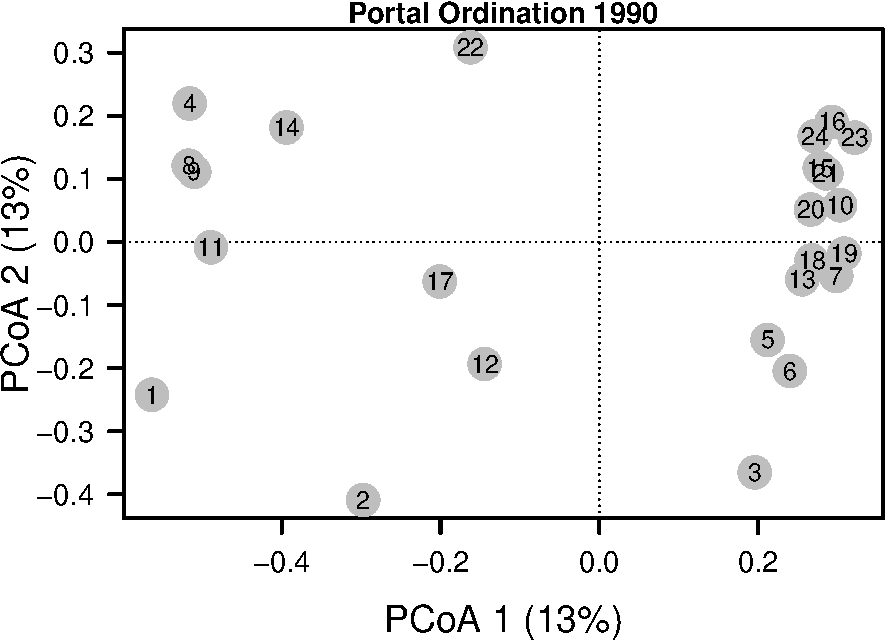
\includegraphics{temporal_assignment_files/figure-latex/unnamed-chunk-3-1.pdf}

\begin{Shaded}
\begin{Highlighting}[]
\CommentTok{#5. Using the hypothesis testing tools you learned in the beta-diversity module, test the hypothesis that species abundances across sites vary as a factor of treatment type (i.e., plot_type)}

\NormalTok{PORTALPERMA}\FloatTok{.90} \NormalTok{=}\StringTok{ }\KeywordTok{adonis}\NormalTok{(portal_90_sbys  ~}\StringTok{ }\NormalTok{ptype, }\DataTypeTok{method =} \StringTok{"bray"}\NormalTok{, }\DataTypeTok{permutations =} \DecValTok{999}\NormalTok{)}
\NormalTok{PORTALPERMA}\FloatTok{.90}
\end{Highlighting}
\end{Shaded}

\begin{verbatim}
## 
## Call:
## adonis(formula = portal_90_sbys ~ ptype, permutations = 999,      method = "bray") 
## 
## Permutation: free
## Number of permutations: 999
## 
## Terms added sequentially (first to last)
## 
##           Df SumsOfSqs MeanSqs F.Model      R2 Pr(>F)    
## ptype      4    2.8656 0.71640  5.8206 0.55064  0.001 ***
## Residuals 19    2.3385 0.12308         0.44936           
## Total     23    5.2041                 1.00000           
## ---
## Signif. codes:  0 '***' 0.001 '**' 0.01 '*' 0.05 '.' 0.1 ' ' 1
\end{verbatim}

\textbf{\emph{Question 2}}: Describe how different biodiversity
estimates vary among sites.

\begin{enumerate}
\def\labelenumi{\alph{enumi}.}
\tightlist
\item
  Does diversity vary among sites? Does this correspond to treatment
  type?
\item
  Is treatment type a significant predictor of site dissimilarity?
\end{enumerate}

\begin{quote}
\textbf{\emph{Answer 2a}}: Diveristy appears to differ among sites. The
PCoA plot shows that the majority of conrtol sites are grouped on the
left side of the plot. \textbf{\emph{Answer 2b}}: Plot treatment type is
a significant predictor of site dissimilarity (P=0.001, R2 = 0.55)
\end{quote}

\subsection{4) TIME SERIES ANALYSIS}\label{time-series-analysis}

In the R code chunk below, do the following:

\begin{enumerate}
\def\labelenumi{\arabic{enumi}.}
\tightlist
\item
  Create a time-by-species matrix that includes year, month, and
  plot\_id for a site other than plot\_id 2.
\item
  Examine per-hectare rodent abundance using simple moving average
  smoothing.
\item
  Test whether your data meets the assumption of stationarity.
\item
  If it does not meet this asumption, explore wasy to make your data
  stationary.
\item
  Examine and plot time lags using the partial autocorrelation function
  (PACF) and autocorrelation function (ACR).
\item
  Use the tools outlined in the Handout to create an ARMA model.
\end{enumerate}

\begin{Shaded}
\begin{Highlighting}[]
\CommentTok{# 1. Create a time-by-species matrix that includes year, month, and plot_id for a site other than plot_id 2.}
\CommentTok{# Make a date vector that contains year, month, and day}
\NormalTok{portal =}\StringTok{ }\KeywordTok{unite}\NormalTok{(portal, }\DataTypeTok{col =} \NormalTok{date, }\KeywordTok{c}\NormalTok{(year, month, day), }\DataTypeTok{sep =} \StringTok{"-"}\NormalTok{, }\DataTypeTok{remove =} \OtherTok{FALSE}\NormalTok{)}

\CommentTok{# Make a taxon vector that contains genus and species names}
\NormalTok{portal =}\StringTok{ }\KeywordTok{unite}\NormalTok{(portal, }\DataTypeTok{col =} \NormalTok{taxon, }\KeywordTok{c}\NormalTok{(genus, species), }\DataTypeTok{sep =} \StringTok{"_"}\NormalTok{, }\DataTypeTok{remove =} \OtherTok{FALSE}\NormalTok{)}

\NormalTok{time.by.species =}\StringTok{ }\NormalTok{portal %>%}\StringTok{  }
\StringTok{                  }\KeywordTok{group_by}\NormalTok{(year, plot_id) %>%}\StringTok{ }
\StringTok{                  }\KeywordTok{count}\NormalTok{(taxon) %>%}\StringTok{ }
\StringTok{                  }\KeywordTok{spread}\NormalTok{(}\DataTypeTok{key =} \NormalTok{taxon, }\DataTypeTok{value =} \NormalTok{n, }\DataTypeTok{fill =} \DecValTok{0}\NormalTok{)}
 
\KeywordTok{filter}\NormalTok{(time.by.species, year ==}\StringTok{ }\DecValTok{1984}\NormalTok{)}
\end{Highlighting}
\end{Shaded}

\begin{verbatim}
## Source: local data frame [24 x 50]
## Groups: year, plot_id [24]
## 
##     year plot_id Ammodramus_savannarum Ammospermophilus_harrisi
##    <int>   <int>                 <dbl>                    <dbl>
## 1   1984       1                     0                        0
## 2   1984       2                     0                        0
## 3   1984       3                     0                        0
## 4   1984       4                     0                        0
## 5   1984       5                     0                        0
## 6   1984       6                     0                        0
## 7   1984       7                     0                        0
## 8   1984       8                     0                        0
## 9   1984       9                     0                        1
## 10  1984      10                     0                        0
## # ... with 14 more rows, and 46 more variables:
## #   Amphispiza_bilineata <dbl>, Baiomys_taylori <dbl>,
## #   Calamospiza_melanocorys <dbl>, Callipepla_squamata <dbl>,
## #   Campylorhynchus_brunneicapillus <dbl>, Chaetodipus_baileyi <dbl>,
## #   Chaetodipus_intermedius <dbl>, Chaetodipus_penicillatus <dbl>,
## #   Chaetodipus_sp. <dbl>, Cnemidophorus_tigris <dbl>,
## #   Cnemidophorus_uniparens <dbl>, Crotalus_scutalatus <dbl>,
## #   Crotalus_viridis <dbl>, Dipodomys_merriami <dbl>,
## #   Dipodomys_ordii <dbl>, Dipodomys_sp. <dbl>,
## #   Dipodomys_spectabilis <dbl>, Lizard_sp. <dbl>, Neotoma_albigula <dbl>,
## #   Onychomys_leucogaster <dbl>, Onychomys_sp. <dbl>,
## #   Onychomys_torridus <dbl>, Perognathus_flavus <dbl>,
## #   Perognathus_hispidus <dbl>, Peromyscus_eremicus <dbl>,
## #   Peromyscus_leucopus <dbl>, Peromyscus_maniculatus <dbl>,
## #   Pipilo_chlorurus <dbl>, Pipilo_fuscus <dbl>, Pipilo_sp. <dbl>,
## #   Pooecetes_gramineus <dbl>, Reithrodontomys_fulvescens <dbl>,
## #   Reithrodontomys_megalotis <dbl>, Reithrodontomys_montanus <dbl>,
## #   Reithrodontomys_sp. <dbl>, Rodent_sp. <dbl>, Sceloporus_clarki <dbl>,
## #   Sceloporus_undulatus <dbl>, Sigmodon_fulviventer <dbl>,
## #   Sigmodon_hispidus <dbl>, Sigmodon_ochrognathus <dbl>,
## #   Sparrow_sp. <dbl>, Spermophilus_spilosoma <dbl>,
## #   Spermophilus_tereticaudus <dbl>, Sylvilagus_audubonii <dbl>,
## #   Zonotrichia_leucophrys <dbl>
\end{verbatim}

\begin{Shaded}
\begin{Highlighting}[]
\KeywordTok{filter}\NormalTok{(time.by.species, plot_id ==}\StringTok{ }\DecValTok{5}\NormalTok{)}
\end{Highlighting}
\end{Shaded}

\begin{verbatim}
## Source: local data frame [26 x 50]
## Groups: year, plot_id [26]
## 
##     year plot_id Ammodramus_savannarum Ammospermophilus_harrisi
##    <int>   <int>                 <dbl>                    <dbl>
## 1   1977       5                     0                        0
## 2   1978       5                     0                        0
## 3   1979       5                     0                        0
## 4   1980       5                     0                        0
## 5   1981       5                     0                        0
## 6   1982       5                     0                        0
## 7   1983       5                     0                        0
## 8   1984       5                     0                        0
## 9   1985       5                     0                        0
## 10  1986       5                     0                        0
## # ... with 16 more rows, and 46 more variables:
## #   Amphispiza_bilineata <dbl>, Baiomys_taylori <dbl>,
## #   Calamospiza_melanocorys <dbl>, Callipepla_squamata <dbl>,
## #   Campylorhynchus_brunneicapillus <dbl>, Chaetodipus_baileyi <dbl>,
## #   Chaetodipus_intermedius <dbl>, Chaetodipus_penicillatus <dbl>,
## #   Chaetodipus_sp. <dbl>, Cnemidophorus_tigris <dbl>,
## #   Cnemidophorus_uniparens <dbl>, Crotalus_scutalatus <dbl>,
## #   Crotalus_viridis <dbl>, Dipodomys_merriami <dbl>,
## #   Dipodomys_ordii <dbl>, Dipodomys_sp. <dbl>,
## #   Dipodomys_spectabilis <dbl>, Lizard_sp. <dbl>, Neotoma_albigula <dbl>,
## #   Onychomys_leucogaster <dbl>, Onychomys_sp. <dbl>,
## #   Onychomys_torridus <dbl>, Perognathus_flavus <dbl>,
## #   Perognathus_hispidus <dbl>, Peromyscus_eremicus <dbl>,
## #   Peromyscus_leucopus <dbl>, Peromyscus_maniculatus <dbl>,
## #   Pipilo_chlorurus <dbl>, Pipilo_fuscus <dbl>, Pipilo_sp. <dbl>,
## #   Pooecetes_gramineus <dbl>, Reithrodontomys_fulvescens <dbl>,
## #   Reithrodontomys_megalotis <dbl>, Reithrodontomys_montanus <dbl>,
## #   Reithrodontomys_sp. <dbl>, Rodent_sp. <dbl>, Sceloporus_clarki <dbl>,
## #   Sceloporus_undulatus <dbl>, Sigmodon_fulviventer <dbl>,
## #   Sigmodon_hispidus <dbl>, Sigmodon_ochrognathus <dbl>,
## #   Sparrow_sp. <dbl>, Spermophilus_spilosoma <dbl>,
## #   Spermophilus_tereticaudus <dbl>, Sylvilagus_audubonii <dbl>,
## #   Zonotrichia_leucophrys <dbl>
\end{verbatim}

\begin{Shaded}
\begin{Highlighting}[]
\NormalTok{time.by.species =}\StringTok{ }\KeywordTok{as.data.frame}\NormalTok{(time.by.species)}

\CommentTok{# 2. Examine per-hectare rodent abundance using simple moving average smoothing.}
\CommentTok{# Create a time-by-species matrix that includes year, month, and plot_id}
\NormalTok{time.by.spec}\FloatTok{.2} \NormalTok{=}\StringTok{ }\KeywordTok{filter}\NormalTok{(portal, taxa==}\StringTok{"Rodent"}\NormalTok{) %>%}\StringTok{ }
\StringTok{                 }\KeywordTok{group_by}\NormalTok{(year, month, plot_id) %>%}
\StringTok{                 }\KeywordTok{count}\NormalTok{(taxon)}
\CommentTok{# Create a seasonality variable using month number (6 = June; 10 = October)}
\NormalTok{time.by.spec}\FloatTok{.2}\NormalTok{$season =}\StringTok{ }\OtherTok{NA}
\NormalTok{time.by.spec}\FloatTok{.2}\NormalTok{$season =}\StringTok{ }\NormalTok{time.by.spec}\FloatTok{.2}\NormalTok{$month %in%}\StringTok{ }\KeywordTok{c}\NormalTok{(}\DecValTok{6}\NormalTok{:}\DecValTok{10}\NormalTok{)}
\CommentTok{# Rainy seasons are June - October}
\NormalTok{time.by.spec}\FloatTok{.2}\NormalTok{$season =}\StringTok{ }\KeywordTok{ifelse}\NormalTok{(time.by.spec}\FloatTok{.2}\NormalTok{$season ==}\StringTok{ }\OtherTok{TRUE}\NormalTok{, }\StringTok{"rain"}\NormalTok{, }\StringTok{"norain"}\NormalTok{)}
\CommentTok{# Group the data by year and season}
\KeywordTok{group_by}\NormalTok{(time.by.spec}\FloatTok{.2}\NormalTok{, year, season)}
\end{Highlighting}
\end{Shaded}

\begin{verbatim}
## Source: local data frame [16,391 x 6]
## Groups: year, season [52]
## 
##     year month plot_id                    taxon     n season
##    <int> <int>   <int>                    <chr> <int>  <chr>
## 1   1977     7       1       Dipodomys_merriami     2   rain
## 2   1977     7       1       Perognathus_flavus     1   rain
## 3   1977     7       2 Chaetodipus_penicillatus     1   rain
## 4   1977     7       2       Dipodomys_merriami     1   rain
## 5   1977     7       2         Neotoma_albigula     1   rain
## 6   1977     7       2      Peromyscus_eremicus     1   rain
## 7   1977     7       3       Dipodomys_merriami     2   rain
## 8   1977     7       3    Dipodomys_spectabilis     1   rain
## 9   1977     7       3         Neotoma_albigula     1   rain
## 10  1977     7       4       Dipodomys_merriami     1   rain
## # ... with 16,381 more rows
\end{verbatim}

\begin{Shaded}
\begin{Highlighting}[]
\NormalTok{abund =}\StringTok{ }\KeywordTok{filter}\NormalTok{(time.by.spec}\FloatTok{.2}\NormalTok{, plot_id ==}\StringTok{ }\DecValTok{2}\NormalTok{) %>%}\StringTok{ }\KeywordTok{group_by}\NormalTok{(year, season) %>%}
\KeywordTok{count}\NormalTok{(}\DataTypeTok{wt =} \NormalTok{n)}
\NormalTok{abund$nn =}\StringTok{ }\NormalTok{abund$nn *}\StringTok{ }\DecValTok{4}
\NormalTok{abund.ts =}\StringTok{ }\KeywordTok{ts}\NormalTok{(abund$nn, }\DataTypeTok{frequency =} \DecValTok{2}\NormalTok{, }\DataTypeTok{start =} \KeywordTok{c}\NormalTok{(}\DecValTok{1977}\NormalTok{, }\DecValTok{2}\NormalTok{))}
\KeywordTok{plot.ts}\NormalTok{(abund.ts, }\DataTypeTok{type =} \StringTok{"l"}\NormalTok{, }\DataTypeTok{ylab =} \StringTok{"Rodent Abundance (#/hectare)"}\NormalTok{, }\DataTypeTok{xlab =} \StringTok{"Time (year)"}\NormalTok{, }\DataTypeTok{las =} \DecValTok{1}\NormalTok{, }\DataTypeTok{ylim =} \KeywordTok{c}\NormalTok{(}\DecValTok{0}\NormalTok{, }\DecValTok{500}\NormalTok{))}
\end{Highlighting}
\end{Shaded}

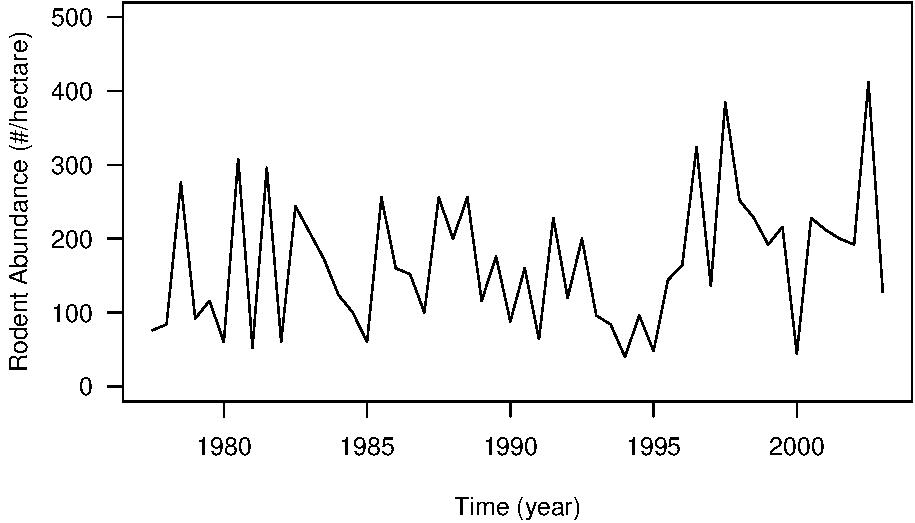
\includegraphics{temporal_assignment_files/figure-latex/unnamed-chunk-4-1.pdf}

\begin{Shaded}
\begin{Highlighting}[]
\CommentTok{# Adding the moving average}
\NormalTok{abund.sm =}\StringTok{ }\KeywordTok{SMA}\NormalTok{(abund$nn, }\DataTypeTok{n =} \DecValTok{4}\NormalTok{)}
\KeywordTok{plot}\NormalTok{(abund.sm, }\DataTypeTok{type =} \StringTok{"l"}\NormalTok{, }\DataTypeTok{col =} \StringTok{"red"}\NormalTok{, }\DataTypeTok{ylab =} \StringTok{"Rodent Abundance (#/hectare)"}\NormalTok{,}
\DataTypeTok{xlab =} \StringTok{"Sample"}\NormalTok{, }\DataTypeTok{las =} \DecValTok{1}\NormalTok{, }\DataTypeTok{ylim =} \KeywordTok{c}\NormalTok{(}\DecValTok{0}\NormalTok{, }\DecValTok{500}\NormalTok{)) }
\KeywordTok{lines}\NormalTok{(abund$nn, }\DataTypeTok{col =} \StringTok{"black"}\NormalTok{)}
\KeywordTok{legend}\NormalTok{(}\DecValTok{0}\NormalTok{, }\DecValTok{475}\NormalTok{, }\DataTypeTok{col =} \KeywordTok{c}\NormalTok{(}\StringTok{"red"}\NormalTok{, }\StringTok{"black"}\NormalTok{), }\DataTypeTok{lty =} \KeywordTok{c}\NormalTok{(}\DecValTok{1}\NormalTok{,}\DecValTok{1}\NormalTok{),}
\KeywordTok{c}\NormalTok{(}\StringTok{"smooth"}\NormalTok{, }\StringTok{"non-smooth"}\NormalTok{), }\DataTypeTok{bty =} \StringTok{"n"}\NormalTok{, }\DataTypeTok{cex =} \DecValTok{1}\NormalTok{)}
\end{Highlighting}
\end{Shaded}

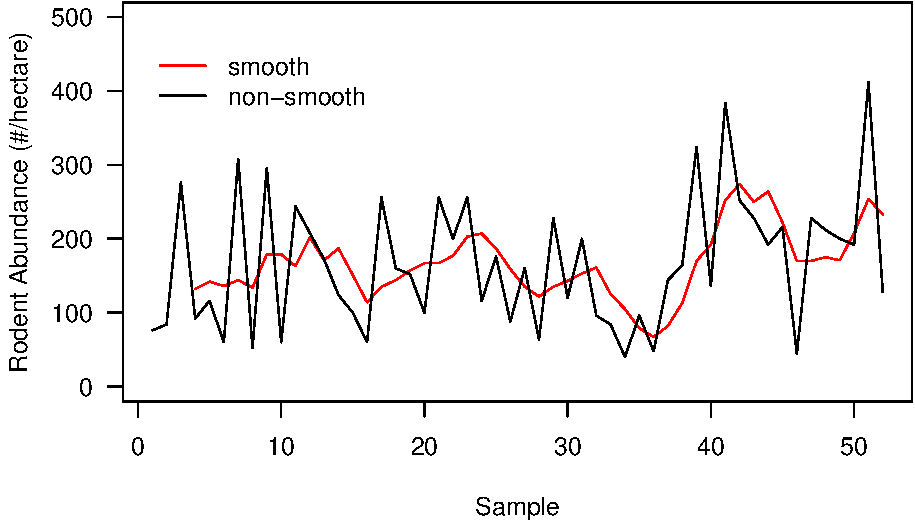
\includegraphics{temporal_assignment_files/figure-latex/unnamed-chunk-4-2.pdf}

\begin{Shaded}
\begin{Highlighting}[]
\CommentTok{# The Holt-Winters filtering technique is commonly used for exponential smoothing}
\NormalTok{abund.hw =}\StringTok{ }\KeywordTok{HoltWinters}\NormalTok{(abund$nn, }\DataTypeTok{beta =} \OtherTok{FALSE}\NormalTok{, }\DataTypeTok{gamma =} \OtherTok{FALSE}\NormalTok{) }
\NormalTok{abund.hw$fitted}
\end{Highlighting}
\end{Shaded}

\begin{verbatim}
## Time Series:
## Start = 2 
## End = 52 
## Frequency = 1 
##         xhat     level
##  2  76.00000  76.00000
##  3  77.16537  77.16537
##  4 106.12982 106.12982
##  5 104.07152 104.07152
##  6 105.80915 105.80915
##  7  99.13608  99.13608
##  8 129.56151 129.56151
##  9 118.26305 118.26305
## 10 144.15418 144.15418
## 11 131.89535 131.89535
## 12 148.22575 148.22575
## 13 156.93313 156.93313
## 14 159.12794 159.12794
## 15 154.01081 154.01081
## 16 146.14300 146.14300
## 17 133.59446 133.59446
## 18 151.42540 151.42540
## 19 152.67448 152.67448
## 20 152.57622 152.57622
## 21 144.91739 144.91739
## 22 161.09891 161.09891
## 23 166.76568 166.76568
## 24 179.76454 179.76454
## 25 170.47589 170.47589
## 26 171.28059 171.28059
## 27 159.14902 159.14902
## 28 159.27298 159.27298
## 29 145.39446 145.39446
## 30 157.42770 157.42770
## 31 151.97557 151.97557
## 32 158.97134 158.97134
## 33 149.79824 149.79824
## 34 140.21334 140.21334
## 35 125.61515 125.61515
## 36 121.30108 121.30108
## 37 110.62323 110.62323
## 38 115.48526 115.48526
## 39 122.55246 122.55246
## 40 151.89754 151.89754
## 41 149.58173 149.58173
## 42 183.72969 183.72969
## 43 193.67470 193.67470
## 44 198.67490 198.67490
## 45 197.70256 197.70256
## 46 200.36797 200.36797
## 47 177.58968 177.58968
## 48 184.93300 184.93300
## 49 188.87588 188.87588
## 50 190.49634 190.49634
## 51 190.71538 190.71538
## 52 222.95015 222.95015
\end{verbatim}

\begin{Shaded}
\begin{Highlighting}[]
\KeywordTok{plot}\NormalTok{(abund.hw, }\DataTypeTok{xlab =} \StringTok{"Time (year)"}\NormalTok{, }\DataTypeTok{ylim =} \KeywordTok{c}\NormalTok{(}\DecValTok{0}\NormalTok{, }\DecValTok{500}\NormalTok{),}
\DataTypeTok{ylab =} \StringTok{"Rodent Abundance (#/hectrare)"}\NormalTok{, }\DataTypeTok{las =} \DecValTok{1}\NormalTok{, }\DataTypeTok{main =} \OtherTok{NA}\NormalTok{) }
\KeywordTok{legend}\NormalTok{(}\DecValTok{0}\NormalTok{, }\DecValTok{475}\NormalTok{, }\DataTypeTok{col =} \KeywordTok{c}\NormalTok{(}\StringTok{"black"}\NormalTok{, }\StringTok{"red"}\NormalTok{), }\DataTypeTok{lty =} \KeywordTok{c}\NormalTok{(}\DecValTok{1}\NormalTok{,}\DecValTok{1}\NormalTok{), }\KeywordTok{c}\NormalTok{(}\StringTok{"non-smooth"}\NormalTok{, }\StringTok{"smooth"}\NormalTok{), }\DataTypeTok{bty =} \StringTok{"n"}\NormalTok{, }\DataTypeTok{cex =} \DecValTok{1}\NormalTok{)}
\end{Highlighting}
\end{Shaded}

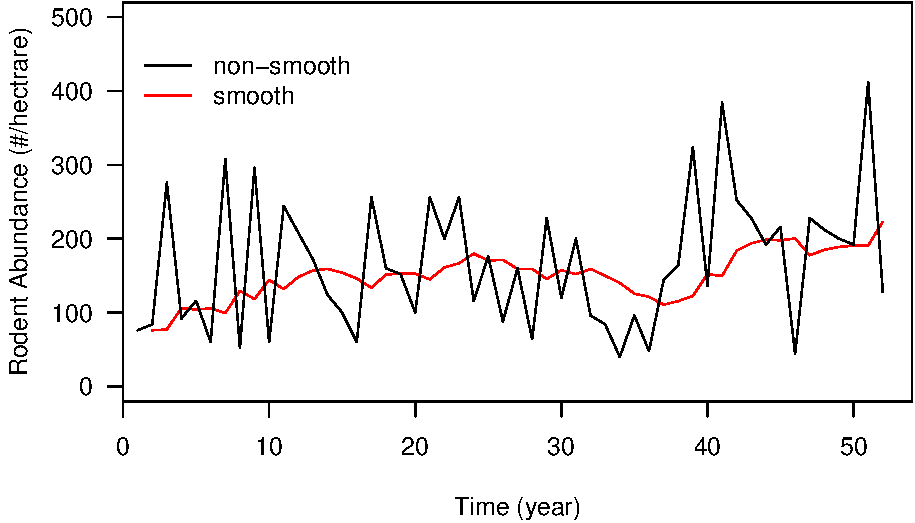
\includegraphics{temporal_assignment_files/figure-latex/unnamed-chunk-4-3.pdf}

\begin{Shaded}
\begin{Highlighting}[]
\CommentTok{# 3. Test whether your data meets the assumption of stationarity.}
\NormalTok{adf.raw =}\StringTok{ }\KeywordTok{adf.test}\NormalTok{(abund.ts, }\DataTypeTok{alternative =} \StringTok{"stationary"}\NormalTok{) }
\NormalTok{adf.raw$p.value}
\end{Highlighting}
\end{Shaded}

\begin{verbatim}
## [1] 0.3229509
\end{verbatim}

\begin{Shaded}
\begin{Highlighting}[]
\NormalTok{abund.ts.diff =}\StringTok{ }\KeywordTok{diff}\NormalTok{(abund.ts)}
\NormalTok{adf.diff =}\StringTok{ }\KeywordTok{adf.test}\NormalTok{(abund.ts.diff, }\DataTypeTok{alternative =} \StringTok{"stationary"}\NormalTok{) }
\NormalTok{adf.diff$p.value}
\end{Highlighting}
\end{Shaded}

\begin{verbatim}
## [1] 0.02186602
\end{verbatim}

\begin{Shaded}
\begin{Highlighting}[]
\CommentTok{#  5. Examine and plot time lags using the partial autocorrelation function (PACF) and autocorrelation function (ACR).}
\KeywordTok{acf}\NormalTok{(abund.ts)}
\end{Highlighting}
\end{Shaded}

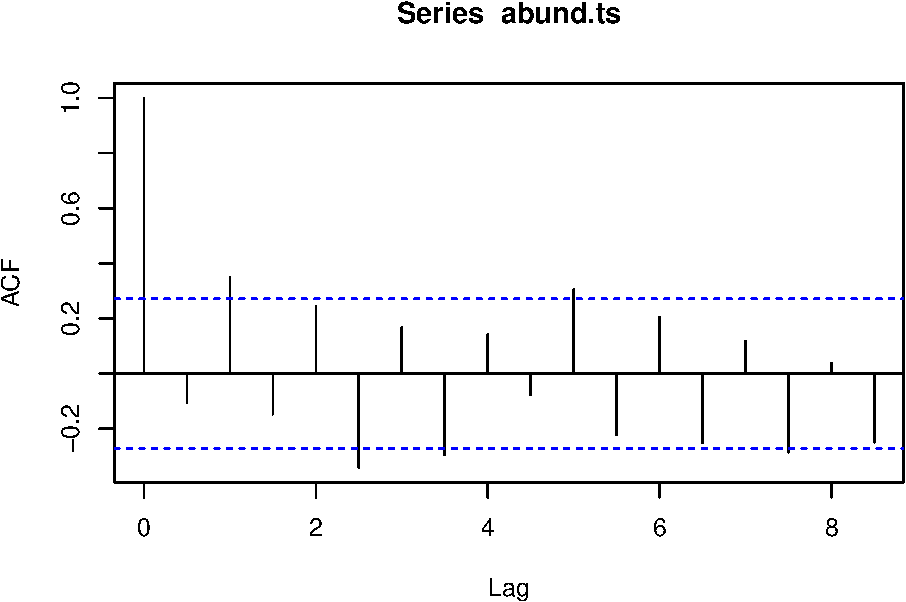
\includegraphics{temporal_assignment_files/figure-latex/unnamed-chunk-4-4.pdf}

\begin{Shaded}
\begin{Highlighting}[]
\KeywordTok{pacf}\NormalTok{(abund.ts)}
\end{Highlighting}
\end{Shaded}

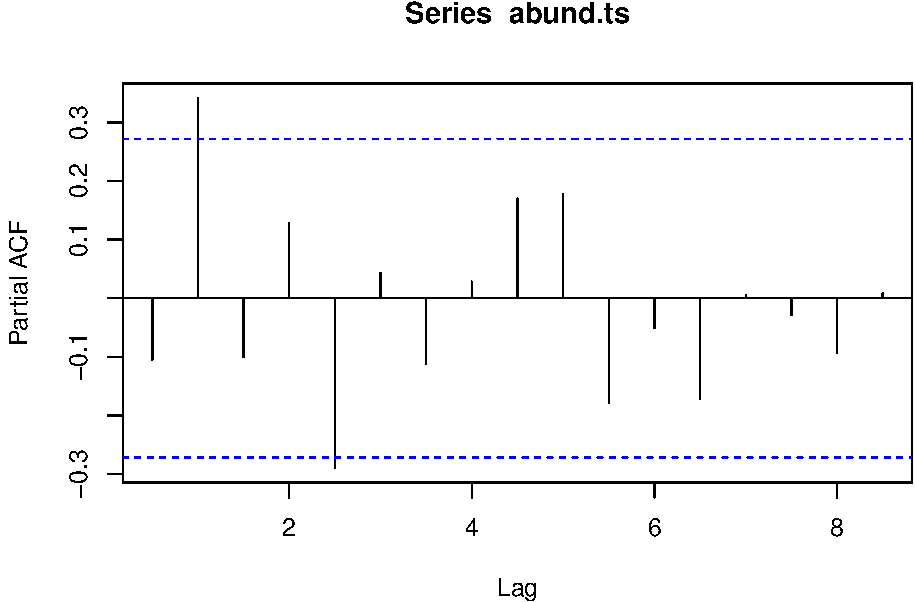
\includegraphics{temporal_assignment_files/figure-latex/unnamed-chunk-4-5.pdf}

\begin{Shaded}
\begin{Highlighting}[]
\CommentTok{# 6. Use the tools outlined in the Handout to create an ARMA model.}
\NormalTok{abund.arm =}\StringTok{ }\KeywordTok{auto.arima}\NormalTok{(abund.ts)}
\NormalTok{abund.arm =}\StringTok{ }\KeywordTok{arima}\NormalTok{((abund.ts), }\KeywordTok{c}\NormalTok{(}\DecValTok{0}\NormalTok{, }\DecValTok{0}\NormalTok{, }\DecValTok{1}\NormalTok{), }\DataTypeTok{seasonal =} \KeywordTok{list}\NormalTok{(}\DataTypeTok{order =} \KeywordTok{c}\NormalTok{(}\DecValTok{2}\NormalTok{, }\DecValTok{1}\NormalTok{, }\DecValTok{0}\NormalTok{),}
                  \DataTypeTok{period =} \DecValTok{2}\NormalTok{), }\DataTypeTok{include.mean =} \OtherTok{TRUE}\NormalTok{)}
\KeywordTok{tsdiag}\NormalTok{(abund.arm)}
\end{Highlighting}
\end{Shaded}

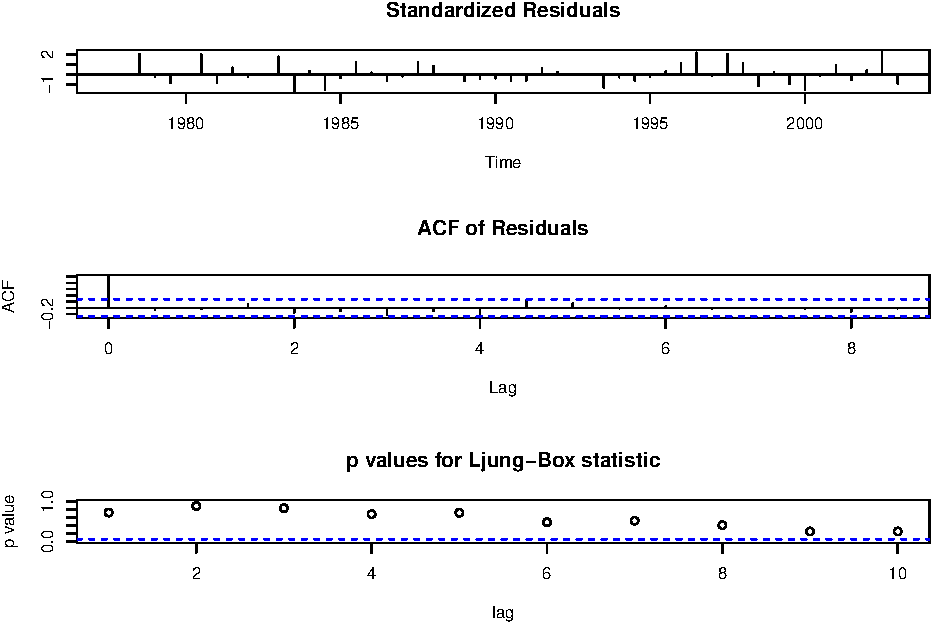
\includegraphics{temporal_assignment_files/figure-latex/unnamed-chunk-4-6.pdf}

\begin{Shaded}
\begin{Highlighting}[]
\NormalTok{pred.arm =}\StringTok{ }\KeywordTok{predict}\NormalTok{(abund.arm, }\DataTypeTok{n.ahead =} \DecValTok{20}\NormalTok{) }
\KeywordTok{ts.plot}\NormalTok{(abund.ts, pred.arm$pred, }\DataTypeTok{lty =} \KeywordTok{c}\NormalTok{(}\DecValTok{1}\NormalTok{,}\DecValTok{3}\NormalTok{))}
\end{Highlighting}
\end{Shaded}

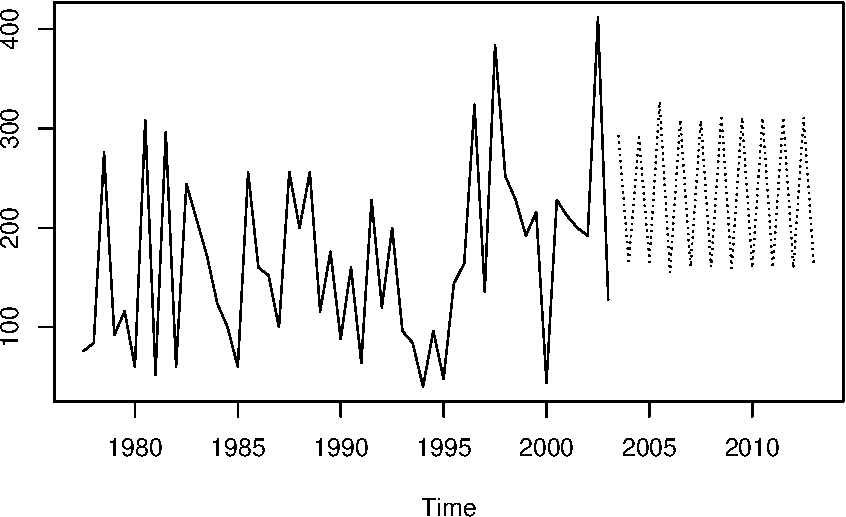
\includegraphics{temporal_assignment_files/figure-latex/unnamed-chunk-4-7.pdf}

\textbf{\emph{Question 3}}: Describe the results from your time series
analysis.

\begin{enumerate}
\def\labelenumi{\alph{enumi}.}
\tightlist
\item
  Does your data meet the assumption of stationarity? If not, what does
  this violation imply?
\item
  What does the ACF function do and how does it relate to the ARMA
  model? How does this differ from the autocorrelation function (ACF)?
\item
  What results can you conclude from your full ARMA model along with
  other methods outlined in the time series setcion of the Handout?
\end{enumerate}

\begin{quote}
\textbf{\emph{Answer 3a}}:The Dickey-Fuller test indicates that our data
does not meet the assumption of stationarity (P\textgreater{}0.05). This
violation implies that the mean, variance and covariance of the time
series is affected by time (i.e.~changes in rodent abundance over time
are affected by seasonal variation in precipitation).
\end{quote}

\begin{quote}
\textbf{\emph{Answer 3b}}:The ACF function allows us to look at the lags
in our time series analysis, specifically the lags of the forecast
errors in relation to the moving average component of the ARMA model.
The ACF tells us about the correlations between lag intervals in the
time series. The correlations should decrease with increasing time lag-
meaning that past values have less of an effect on current values. We
are also using the partial autocorrelation function (PACF) in addition
to the ACF function. In contrast to the ACF, the PACF tells us about
lags that can be addressed with the autoregressive component of the ARMA
model.
\end{quote}

\begin{quote}
\textbf{\emph{Answer 3c}}:The ACF tells us that there is a significant
positive correlation at time lag 2- indicative of the annual
precipitation cycle (rainy vs.~non rainy season). Differencing the data
allowed us to meet the assumptions of stationarity and therefore we can
use a autoregressive integrated moving average (ARIMA) model to to
remove the effect of time lag 2. Looking at the diagnostic plots for the
ARIMA model, we have removed the seasonal trend in abundances due to
precipitation. Forecasting rodent abundances in the future for the study
plot, we can see that abundances will fluctuate around 250 and
abundances will be less variable than in previous years.
\end{quote}

\subsection{5) REPEATED MEASURES ANALYSIS OF VARIANCE
(RM-ANOVA)}\label{repeated-measures-analysis-of-variance-rm-anova}

In the R code chunk below, do the following:

\begin{enumerate}
\def\labelenumi{\arabic{enumi}.}
\tightlist
\item
  Create an appropriate data frame for RM-ANOVA (e.g., yearly species
  abundance values within plots).
\item
  Calculate the inverse of Simpson's diversity for each year, and plot
  it as a function of year for the Control and Rodent Exclosure plots.
\item
  Perform an RM-ANOVA and construct a F-test using the AR(1), compound
  symmetery, and unstructured covariance structures.
\end{enumerate}

\begin{Shaded}
\begin{Highlighting}[]
\CommentTok{# Construct time-by-species matrix}
\NormalTok{time.by.species =}\StringTok{ }\NormalTok{portal %>%}
\StringTok{                  }\KeywordTok{group_by}\NormalTok{(year, plot_id,plot_type) %>%}\StringTok{ }
\StringTok{                  }\KeywordTok{count}\NormalTok{(taxon) %>%}\StringTok{ }
\StringTok{                  }\KeywordTok{spread}\NormalTok{(}\DataTypeTok{key =} \NormalTok{taxon, }\DataTypeTok{value =} \NormalTok{n, }\DataTypeTok{fill =} \DecValTok{0}\NormalTok{)}
\CommentTok{# 2. Calculate the inverse of Simpson's diversity for each year, and plot it as a function of year for the Control and Rodent Exclosure plots.}

\CommentTok{# Calculating Simpsons diversity index}
\NormalTok{insimp =}\StringTok{ }\KeywordTok{diversity}\NormalTok{(time.by.species[,-}\KeywordTok{c}\NormalTok{(}\DecValTok{1}\NormalTok{:}\DecValTok{3}\NormalTok{)], }\StringTok{"invsimpson"}\NormalTok{)}

\CommentTok{# Create data frame with experimental design and diversity data}
\NormalTok{div.all =}\StringTok{ }\KeywordTok{data.frame}\NormalTok{(time.by.species[,}\DecValTok{1}\NormalTok{:}\DecValTok{3}\NormalTok{,], insimp)}
\CommentTok{# Rename column}
\KeywordTok{names}\NormalTok{(div.all)[}\DecValTok{4}\NormalTok{] =}\StringTok{ "inv.simp"}
\CommentTok{# Pull out two of the five Portal treatments}
\NormalTok{div.treat =}\StringTok{ }\NormalTok{div.all[}\KeywordTok{which}\NormalTok{(div.all$plot_type ==}
\StringTok{"Control"} \NormalTok{|}\StringTok{ }\NormalTok{div.all$plot_type ==}\StringTok{ "Rodent Exclosure"}\NormalTok{), ]}

\NormalTok{div.treat.plot =}\StringTok{ }\KeywordTok{group_by}\NormalTok{(div.treat, plot_type, year) %>%}
\StringTok{  }\KeywordTok{summarise}\NormalTok{(}\DataTypeTok{mean =} \KeywordTok{mean}\NormalTok{(inv.simp), }\DataTypeTok{sd =} \KeywordTok{sd}\NormalTok{(inv.simp),}\DataTypeTok{n =} \KeywordTok{n}\NormalTok{(),}\DataTypeTok{sem =} \NormalTok{sd/}\KeywordTok{sqrt}\NormalTok{(n))}
\CommentTok{# avg. diversity per group}
\CommentTok{# stand. dev. per group}
\CommentTok{# num. obs. per group}
\CommentTok{# calc. std. err. mean.}
\NormalTok{div.plot =}\StringTok{ }\KeywordTok{ggplot}\NormalTok{(div.treat.plot, }\KeywordTok{aes}\NormalTok{(}\DataTypeTok{x =} \NormalTok{year, }\DataTypeTok{y =} \NormalTok{mean, }\DataTypeTok{color =} \NormalTok{plot_type)) +}\StringTok{ }\KeywordTok{geom_line}\NormalTok{(}\DataTypeTok{size =} \DecValTok{1}\NormalTok{, }\DataTypeTok{show.legend =} \NormalTok{T) +}
\StringTok{                  }\KeywordTok{geom_errorbar}\NormalTok{(}\KeywordTok{aes}\NormalTok{(}\DataTypeTok{ymin =} \NormalTok{mean -}\StringTok{ }\NormalTok{sem, }\DataTypeTok{ymax =} \NormalTok{mean +}\StringTok{ }\NormalTok{sem), }\DataTypeTok{width =} \NormalTok{.}\DecValTok{1}\NormalTok{) +}\StringTok{  }\KeywordTok{xlim}\NormalTok{(}\DecValTok{1977}\NormalTok{, }\DecValTok{2002}\NormalTok{) +}\StringTok{ }\KeywordTok{xlab}\NormalTok{(}\StringTok{"Year"}\NormalTok{) +}\StringTok{ }\KeywordTok{ylab}\NormalTok{(}\StringTok{"(1/D) "}\NormalTok{)+}\StringTok{ }\KeywordTok{scale_color_grey}\NormalTok{()}
\KeywordTok{plot}\NormalTok{(div.plot)}
\end{Highlighting}
\end{Shaded}

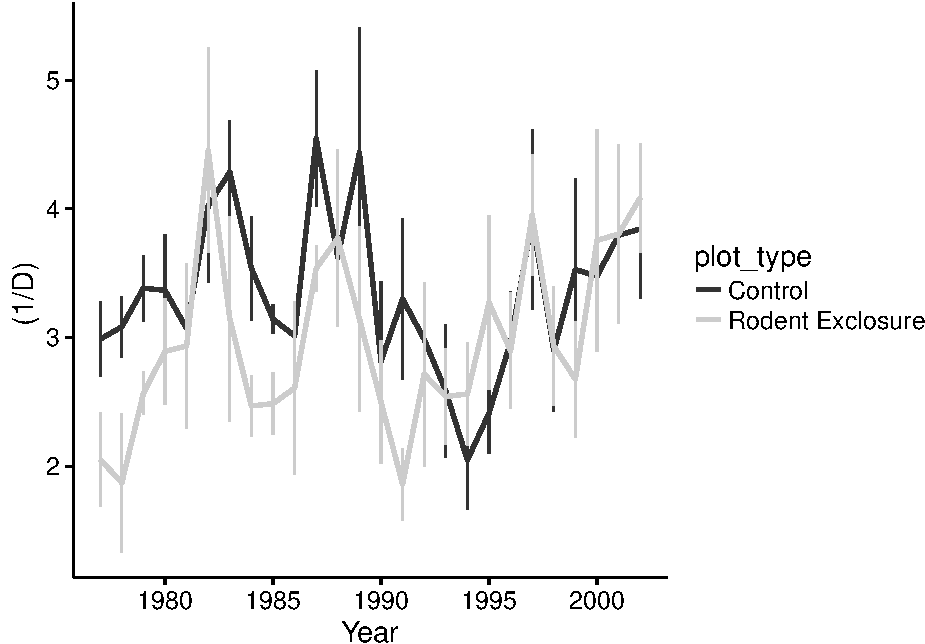
\includegraphics{temporal_assignment_files/figure-latex/unnamed-chunk-5-1.pdf}

\begin{Shaded}
\begin{Highlighting}[]
\CommentTok{# 3. Perform an RM-ANOVA and construct a F-test using the AR(1), compound symmetery, and unstructured covariance structures.}

\CommentTok{# AR(1) covariance structure}
\NormalTok{div.rm1 =}\StringTok{ }\KeywordTok{lme}\NormalTok{(inv.simp ~}\StringTok{ }\NormalTok{plot_type *}\StringTok{ }\NormalTok{year, }\DataTypeTok{random =} \NormalTok{~}\StringTok{ }\DecValTok{1} \NormalTok{|}\StringTok{ }\NormalTok{plot_id, }\DataTypeTok{correlation =} \KeywordTok{corAR1}\NormalTok{(}\DataTypeTok{form =} \NormalTok{~}\StringTok{ }\DecValTok{1} \NormalTok{|}\StringTok{ }\NormalTok{plot_id),}\DataTypeTok{data =} \NormalTok{div.treat) }\CommentTok{# Look at detailed output}
\KeywordTok{summary}\NormalTok{(div.rm1) }\CommentTok{# Obtain F-test}
\end{Highlighting}
\end{Shaded}

\begin{verbatim}
## Linear mixed-effects model fit by REML
##  Data: div.treat 
##        AIC      BIC    logLik
##   1153.217 1180.322 -569.6087
## 
## Random effects:
##  Formula: ~1 | plot_id
##         (Intercept) Residual
## StdDev:   0.6469478 1.250206
## 
## Correlation Structure: AR(1)
##  Formula: ~1 | plot_id 
##  Parameter estimate(s):
##       Phi 
## 0.4250398 
## Fixed effects: inv.simp ~ plot_type * year 
##                                    Value Std.Error  DF    t-value p-value
## (Intercept)                      1.36695  33.32814 343  0.0410150  0.9673
## plot_typeRodent Exclosure      -73.37575  52.01883  12 -1.4105613  0.1838
## year                             0.00100   0.01675 343  0.0595739  0.9525
## plot_typeRodent Exclosure:year   0.03670   0.02614 343  1.4039132  0.1612
##  Correlation: 
##                                (Intr) plt_RE year  
## plot_typeRodent Exclosure      -0.641              
## year                           -1.000  0.641       
## plot_typeRodent Exclosure:year  0.641 -1.000 -0.641
## 
## Standardized Within-Group Residuals:
##         Min          Q1         Med          Q3         Max 
## -1.93162654 -0.70434296 -0.08293334  0.45856267  5.06139168 
## 
## Number of Observations: 359
## Number of Groups: 14
\end{verbatim}

\begin{Shaded}
\begin{Highlighting}[]
\KeywordTok{anova}\NormalTok{(div.rm1)}
\end{Highlighting}
\end{Shaded}

\begin{verbatim}
##                numDF denDF   F-value p-value
## (Intercept)        1   343 256.22009  <.0001
## plot_type          1    12   0.72274  0.4119
## year               1   343   1.56060  0.2124
## plot_type:year     1   343   1.97097  0.1612
\end{verbatim}

\begin{Shaded}
\begin{Highlighting}[]
\CommentTok{# Make cleaner ANOVA table}
\KeywordTok{set.caption}\NormalTok{(}\StringTok{"RMANOVA for Portal Using AR(1) covariance Structure"}\NormalTok{) }
\KeywordTok{pander}\NormalTok{(}\KeywordTok{anova}\NormalTok{(div.rm1))}
\end{Highlighting}
\end{Shaded}

\begin{longtable}[c]{@{}ccccc@{}}
\caption{RMANOVA for Portal Using AR(1) covariance
Structure}\tabularnewline
\toprule
\begin{minipage}[b]{0.25\columnwidth}\centering\strut
~
\strut\end{minipage} &
\begin{minipage}[b]{0.10\columnwidth}\centering\strut
numDF
\strut\end{minipage} &
\begin{minipage}[b]{0.10\columnwidth}\centering\strut
denDF
\strut\end{minipage} &
\begin{minipage}[b]{0.12\columnwidth}\centering\strut
F-value
\strut\end{minipage} &
\begin{minipage}[b]{0.12\columnwidth}\centering\strut
p-value
\strut\end{minipage}\tabularnewline
\midrule
\endfirsthead
\toprule
\begin{minipage}[b]{0.25\columnwidth}\centering\strut
~
\strut\end{minipage} &
\begin{minipage}[b]{0.10\columnwidth}\centering\strut
numDF
\strut\end{minipage} &
\begin{minipage}[b]{0.10\columnwidth}\centering\strut
denDF
\strut\end{minipage} &
\begin{minipage}[b]{0.12\columnwidth}\centering\strut
F-value
\strut\end{minipage} &
\begin{minipage}[b]{0.12\columnwidth}\centering\strut
p-value
\strut\end{minipage}\tabularnewline
\midrule
\endhead
\begin{minipage}[t]{0.25\columnwidth}\centering\strut
\textbf{(Intercept)}
\strut\end{minipage} &
\begin{minipage}[t]{0.10\columnwidth}\centering\strut
1
\strut\end{minipage} &
\begin{minipage}[t]{0.10\columnwidth}\centering\strut
343
\strut\end{minipage} &
\begin{minipage}[t]{0.12\columnwidth}\centering\strut
256.2
\strut\end{minipage} &
\begin{minipage}[t]{0.12\columnwidth}\centering\strut
0
\strut\end{minipage}\tabularnewline
\begin{minipage}[t]{0.25\columnwidth}\centering\strut
\textbf{plot\_type}
\strut\end{minipage} &
\begin{minipage}[t]{0.10\columnwidth}\centering\strut
1
\strut\end{minipage} &
\begin{minipage}[t]{0.10\columnwidth}\centering\strut
12
\strut\end{minipage} &
\begin{minipage}[t]{0.12\columnwidth}\centering\strut
0.7227
\strut\end{minipage} &
\begin{minipage}[t]{0.12\columnwidth}\centering\strut
0.4119
\strut\end{minipage}\tabularnewline
\begin{minipage}[t]{0.25\columnwidth}\centering\strut
\textbf{year}
\strut\end{minipage} &
\begin{minipage}[t]{0.10\columnwidth}\centering\strut
1
\strut\end{minipage} &
\begin{minipage}[t]{0.10\columnwidth}\centering\strut
343
\strut\end{minipage} &
\begin{minipage}[t]{0.12\columnwidth}\centering\strut
1.561
\strut\end{minipage} &
\begin{minipage}[t]{0.12\columnwidth}\centering\strut
0.2124
\strut\end{minipage}\tabularnewline
\begin{minipage}[t]{0.25\columnwidth}\centering\strut
\textbf{plot\_type:year}
\strut\end{minipage} &
\begin{minipage}[t]{0.10\columnwidth}\centering\strut
1
\strut\end{minipage} &
\begin{minipage}[t]{0.10\columnwidth}\centering\strut
343
\strut\end{minipage} &
\begin{minipage}[t]{0.12\columnwidth}\centering\strut
1.971
\strut\end{minipage} &
\begin{minipage}[t]{0.12\columnwidth}\centering\strut
0.1612
\strut\end{minipage}\tabularnewline
\bottomrule
\end{longtable}

\begin{Shaded}
\begin{Highlighting}[]
\CommentTok{# Use `lsmeans` package for time-corrected marginal means}
\KeywordTok{lsmeans}\NormalTok{(div.rm1, ~plot_type)}
\end{Highlighting}
\end{Shaded}

\begin{verbatim}
## NOTE: Results may be misleading due to involvement in interactions
\end{verbatim}

\begin{verbatim}
##  plot_type          lsmean        SE df lower.CL upper.CL
##  Control          3.352478 0.2644674 13 2.781131 3.923825
##  Rodent Exclosure 3.002943 0.3066216 12 2.334872 3.671014
## 
## Confidence level used: 0.95
\end{verbatim}

\begin{Shaded}
\begin{Highlighting}[]
\CommentTok{# compound symmetery covariance structure}
\NormalTok{div.rm2 =}\StringTok{ }\KeywordTok{lme}\NormalTok{(inv.simp ~}\StringTok{ }\NormalTok{plot_type *}\StringTok{ }\NormalTok{year, }\DataTypeTok{random =} \NormalTok{~}\StringTok{ }\DecValTok{1} \NormalTok{|}\StringTok{ }\NormalTok{plot_id, }\DataTypeTok{correlation =} \KeywordTok{corCompSymm}\NormalTok{(}\DataTypeTok{form =} \NormalTok{~}\StringTok{ }\DecValTok{1} \NormalTok{|}\StringTok{ }\NormalTok{plot_id),}\DataTypeTok{data =} \NormalTok{div.treat) }\CommentTok{# Look at detailed output}
\KeywordTok{summary}\NormalTok{(div.rm2) }\CommentTok{# Obtain F-test}
\end{Highlighting}
\end{Shaded}

\begin{verbatim}
## Linear mixed-effects model fit by REML
##  Data: div.treat 
##        AIC      BIC    logLik
##   1215.368 1242.473 -600.6842
## 
## Random effects:
##  Formula: ~1 | plot_id
##         (Intercept) Residual
## StdDev:   0.7104222 1.214275
## 
## Correlation Structure: Compound symmetry
##  Formula: ~1 | plot_id 
##  Parameter estimate(s):
##          Rho 
## 6.672013e-18 
## Fixed effects: inv.simp ~ plot_type * year 
##                                    Value Std.Error  DF    t-value p-value
## (Intercept)                     13.26069  22.33564 343  0.5937008  0.5531
## plot_typeRodent Exclosure      -68.60423  34.97126  12 -1.9617316  0.0734
## year                            -0.00498   0.01123 343 -0.4438008  0.6575
## plot_typeRodent Exclosure:year   0.03431   0.01758 343  1.9518712  0.0518
##  Correlation: 
##                                (Intr) plt_RE year  
## plot_typeRodent Exclosure      -0.639              
## year                           -1.000  0.639       
## plot_typeRodent Exclosure:year  0.639 -1.000 -0.639
## 
## Standardized Within-Group Residuals:
##        Min         Q1        Med         Q3        Max 
## -2.0346517 -0.6823806 -0.1001395  0.4790022  5.1406695 
## 
## Number of Observations: 359
## Number of Groups: 14
\end{verbatim}

\begin{Shaded}
\begin{Highlighting}[]
\KeywordTok{anova}\NormalTok{(div.rm2)}
\end{Highlighting}
\end{Shaded}

\begin{verbatim}
##                numDF denDF   F-value p-value
## (Intercept)        1   343 255.02615  <.0001
## plot_type          1    12   0.73483  0.4081
## year               1   343   1.08893  0.2974
## plot_type:year     1   343   3.80980  0.0518
\end{verbatim}

\begin{Shaded}
\begin{Highlighting}[]
\CommentTok{# Make cleaner ANOVA table}
\KeywordTok{set.caption}\NormalTok{(}\StringTok{"RMANOVA for Portal Using compound symmetry covariance Structure"}\NormalTok{) }
\KeywordTok{pander}\NormalTok{(}\KeywordTok{anova}\NormalTok{(div.rm2))}
\end{Highlighting}
\end{Shaded}

\begin{longtable}[c]{@{}ccccc@{}}
\caption{RMANOVA for Portal Using compound symmetry covariance
Structure}\tabularnewline
\toprule
\begin{minipage}[b]{0.25\columnwidth}\centering\strut
~
\strut\end{minipage} &
\begin{minipage}[b]{0.10\columnwidth}\centering\strut
numDF
\strut\end{minipage} &
\begin{minipage}[b]{0.10\columnwidth}\centering\strut
denDF
\strut\end{minipage} &
\begin{minipage}[b]{0.12\columnwidth}\centering\strut
F-value
\strut\end{minipage} &
\begin{minipage}[b]{0.12\columnwidth}\centering\strut
p-value
\strut\end{minipage}\tabularnewline
\midrule
\endfirsthead
\toprule
\begin{minipage}[b]{0.25\columnwidth}\centering\strut
~
\strut\end{minipage} &
\begin{minipage}[b]{0.10\columnwidth}\centering\strut
numDF
\strut\end{minipage} &
\begin{minipage}[b]{0.10\columnwidth}\centering\strut
denDF
\strut\end{minipage} &
\begin{minipage}[b]{0.12\columnwidth}\centering\strut
F-value
\strut\end{minipage} &
\begin{minipage}[b]{0.12\columnwidth}\centering\strut
p-value
\strut\end{minipage}\tabularnewline
\midrule
\endhead
\begin{minipage}[t]{0.25\columnwidth}\centering\strut
\textbf{(Intercept)}
\strut\end{minipage} &
\begin{minipage}[t]{0.10\columnwidth}\centering\strut
1
\strut\end{minipage} &
\begin{minipage}[t]{0.10\columnwidth}\centering\strut
343
\strut\end{minipage} &
\begin{minipage}[t]{0.12\columnwidth}\centering\strut
255
\strut\end{minipage} &
\begin{minipage}[t]{0.12\columnwidth}\centering\strut
0
\strut\end{minipage}\tabularnewline
\begin{minipage}[t]{0.25\columnwidth}\centering\strut
\textbf{plot\_type}
\strut\end{minipage} &
\begin{minipage}[t]{0.10\columnwidth}\centering\strut
1
\strut\end{minipage} &
\begin{minipage}[t]{0.10\columnwidth}\centering\strut
12
\strut\end{minipage} &
\begin{minipage}[t]{0.12\columnwidth}\centering\strut
0.7348
\strut\end{minipage} &
\begin{minipage}[t]{0.12\columnwidth}\centering\strut
0.4081
\strut\end{minipage}\tabularnewline
\begin{minipage}[t]{0.25\columnwidth}\centering\strut
\textbf{year}
\strut\end{minipage} &
\begin{minipage}[t]{0.10\columnwidth}\centering\strut
1
\strut\end{minipage} &
\begin{minipage}[t]{0.10\columnwidth}\centering\strut
343
\strut\end{minipage} &
\begin{minipage}[t]{0.12\columnwidth}\centering\strut
1.089
\strut\end{minipage} &
\begin{minipage}[t]{0.12\columnwidth}\centering\strut
0.2974
\strut\end{minipage}\tabularnewline
\begin{minipage}[t]{0.25\columnwidth}\centering\strut
\textbf{plot\_type:year}
\strut\end{minipage} &
\begin{minipage}[t]{0.10\columnwidth}\centering\strut
1
\strut\end{minipage} &
\begin{minipage}[t]{0.10\columnwidth}\centering\strut
343
\strut\end{minipage} &
\begin{minipage}[t]{0.12\columnwidth}\centering\strut
3.81
\strut\end{minipage} &
\begin{minipage}[t]{0.12\columnwidth}\centering\strut
0.05177
\strut\end{minipage}\tabularnewline
\bottomrule
\end{longtable}

\begin{Shaded}
\begin{Highlighting}[]
\CommentTok{# Use `lsmeans` package for time-corrected marginal means}
\KeywordTok{lsmeans}\NormalTok{(div.rm2, ~plot_type)}
\end{Highlighting}
\end{Shaded}

\begin{verbatim}
## NOTE: Results may be misleading due to involvement in interactions
\end{verbatim}

\begin{verbatim}
##  plot_type          lsmean        SE df lower.CL upper.CL
##  Control          3.348317 0.2649103 13 2.776013 3.920621
##  Rodent Exclosure 2.997377 0.3064250 12 2.329735 3.665020
## 
## Confidence level used: 0.95
\end{verbatim}

\begin{Shaded}
\begin{Highlighting}[]
\CommentTok{# unstructured covariance structure}
\NormalTok{div.rm3 =}\StringTok{ }\KeywordTok{lme}\NormalTok{(inv.simp ~}\StringTok{ }\NormalTok{plot_type *year, }\DataTypeTok{random =} \NormalTok{~}\StringTok{ }\DecValTok{1} \NormalTok{|}\StringTok{ }\NormalTok{plot_id, }\DataTypeTok{data =} \NormalTok{div.treat) }
\CommentTok{#Look at detailed output}
\KeywordTok{summary}\NormalTok{(div.rm3) }\CommentTok{# Obtain F-test}
\end{Highlighting}
\end{Shaded}

\begin{verbatim}
## Linear mixed-effects model fit by REML
##  Data: div.treat 
##        AIC      BIC    logLik
##   1213.368 1236.601 -600.6842
## 
## Random effects:
##  Formula: ~1 | plot_id
##         (Intercept) Residual
## StdDev:   0.7104222 1.214275
## 
## Fixed effects: inv.simp ~ plot_type * year 
##                                    Value Std.Error  DF    t-value p-value
## (Intercept)                     13.26069  22.33564 343  0.5937008  0.5531
## plot_typeRodent Exclosure      -68.60423  34.97126  12 -1.9617316  0.0734
## year                            -0.00498   0.01123 343 -0.4438008  0.6575
## plot_typeRodent Exclosure:year   0.03431   0.01758 343  1.9518712  0.0518
##  Correlation: 
##                                (Intr) plt_RE year  
## plot_typeRodent Exclosure      -0.639              
## year                           -1.000  0.639       
## plot_typeRodent Exclosure:year  0.639 -1.000 -0.639
## 
## Standardized Within-Group Residuals:
##        Min         Q1        Med         Q3        Max 
## -2.0346517 -0.6823806 -0.1001395  0.4790022  5.1406695 
## 
## Number of Observations: 359
## Number of Groups: 14
\end{verbatim}

\begin{Shaded}
\begin{Highlighting}[]
\KeywordTok{anova}\NormalTok{(div.rm3)}
\end{Highlighting}
\end{Shaded}

\begin{verbatim}
##                numDF denDF   F-value p-value
## (Intercept)        1   343 255.02615  <.0001
## plot_type          1    12   0.73483  0.4081
## year               1   343   1.08893  0.2974
## plot_type:year     1   343   3.80980  0.0518
\end{verbatim}

\begin{Shaded}
\begin{Highlighting}[]
\CommentTok{# Make cleaner ANOVA table}
\KeywordTok{set.caption}\NormalTok{(}\StringTok{"RMANOVA for Portal Using unstructured covariance Structure"}\NormalTok{) }
\KeywordTok{pander}\NormalTok{(}\KeywordTok{anova}\NormalTok{(div.rm3))}
\end{Highlighting}
\end{Shaded}

\begin{longtable}[c]{@{}ccccc@{}}
\caption{RMANOVA for Portal Using unstructured covariance
Structure}\tabularnewline
\toprule
\begin{minipage}[b]{0.25\columnwidth}\centering\strut
~
\strut\end{minipage} &
\begin{minipage}[b]{0.10\columnwidth}\centering\strut
numDF
\strut\end{minipage} &
\begin{minipage}[b]{0.10\columnwidth}\centering\strut
denDF
\strut\end{minipage} &
\begin{minipage}[b]{0.12\columnwidth}\centering\strut
F-value
\strut\end{minipage} &
\begin{minipage}[b]{0.12\columnwidth}\centering\strut
p-value
\strut\end{minipage}\tabularnewline
\midrule
\endfirsthead
\toprule
\begin{minipage}[b]{0.25\columnwidth}\centering\strut
~
\strut\end{minipage} &
\begin{minipage}[b]{0.10\columnwidth}\centering\strut
numDF
\strut\end{minipage} &
\begin{minipage}[b]{0.10\columnwidth}\centering\strut
denDF
\strut\end{minipage} &
\begin{minipage}[b]{0.12\columnwidth}\centering\strut
F-value
\strut\end{minipage} &
\begin{minipage}[b]{0.12\columnwidth}\centering\strut
p-value
\strut\end{minipage}\tabularnewline
\midrule
\endhead
\begin{minipage}[t]{0.25\columnwidth}\centering\strut
\textbf{(Intercept)}
\strut\end{minipage} &
\begin{minipage}[t]{0.10\columnwidth}\centering\strut
1
\strut\end{minipage} &
\begin{minipage}[t]{0.10\columnwidth}\centering\strut
343
\strut\end{minipage} &
\begin{minipage}[t]{0.12\columnwidth}\centering\strut
255
\strut\end{minipage} &
\begin{minipage}[t]{0.12\columnwidth}\centering\strut
0
\strut\end{minipage}\tabularnewline
\begin{minipage}[t]{0.25\columnwidth}\centering\strut
\textbf{plot\_type}
\strut\end{minipage} &
\begin{minipage}[t]{0.10\columnwidth}\centering\strut
1
\strut\end{minipage} &
\begin{minipage}[t]{0.10\columnwidth}\centering\strut
12
\strut\end{minipage} &
\begin{minipage}[t]{0.12\columnwidth}\centering\strut
0.7348
\strut\end{minipage} &
\begin{minipage}[t]{0.12\columnwidth}\centering\strut
0.4081
\strut\end{minipage}\tabularnewline
\begin{minipage}[t]{0.25\columnwidth}\centering\strut
\textbf{year}
\strut\end{minipage} &
\begin{minipage}[t]{0.10\columnwidth}\centering\strut
1
\strut\end{minipage} &
\begin{minipage}[t]{0.10\columnwidth}\centering\strut
343
\strut\end{minipage} &
\begin{minipage}[t]{0.12\columnwidth}\centering\strut
1.089
\strut\end{minipage} &
\begin{minipage}[t]{0.12\columnwidth}\centering\strut
0.2974
\strut\end{minipage}\tabularnewline
\begin{minipage}[t]{0.25\columnwidth}\centering\strut
\textbf{plot\_type:year}
\strut\end{minipage} &
\begin{minipage}[t]{0.10\columnwidth}\centering\strut
1
\strut\end{minipage} &
\begin{minipage}[t]{0.10\columnwidth}\centering\strut
343
\strut\end{minipage} &
\begin{minipage}[t]{0.12\columnwidth}\centering\strut
3.81
\strut\end{minipage} &
\begin{minipage}[t]{0.12\columnwidth}\centering\strut
0.05177
\strut\end{minipage}\tabularnewline
\bottomrule
\end{longtable}

\begin{Shaded}
\begin{Highlighting}[]
\CommentTok{# Use `lsmeans` package for time-corrected marginal means}
\KeywordTok{lsmeans}\NormalTok{(div.rm3, ~plot_type)}
\end{Highlighting}
\end{Shaded}

\begin{verbatim}
## NOTE: Results may be misleading due to involvement in interactions
\end{verbatim}

\begin{verbatim}
##  plot_type          lsmean        SE df lower.CL upper.CL
##  Control          3.348317 0.2649103 13 2.776013 3.920621
##  Rodent Exclosure 2.997377 0.3064250 12 2.329735 3.665020
## 
## Confidence level used: 0.95
\end{verbatim}

\begin{Shaded}
\begin{Highlighting}[]
\CommentTok{# Compare the AICs}
\KeywordTok{AIC}\NormalTok{(div.rm1, div.rm2, div.rm3)}
\end{Highlighting}
\end{Shaded}

\begin{verbatim}
##         df      AIC
## div.rm1  7 1153.217
## div.rm2  7 1215.368
## div.rm3  6 1213.368
\end{verbatim}

\textbf{\emph{Question 4}}: Describe the results from your RM-ANOVA.

\begin{quote}
\textbf{\emph{Answer 4a}}: The RM-ANOVA allows you to test for the main
effects of treatment, time and a treatment x time interaction by
accounting for the non-independence of observations or the fact that
time points are not independent of one another and that repeated
measurements have been taken for the different plots.
\end{quote}

\begin{quote}
\textbf{\emph{Answer 4b}}: There is no obvious trend for inverse of
Simpson's diversity (1/D) over time. 1/D fluctuates over time and tends
to lower in rodent exlosure experiments in the early part of the study
(1977-1980).
\end{quote}

\begin{quote}
\textbf{\emph{Answer 4c}}:The result of the F-test tells us that year,
plot type and the plot type by year interaction did not have a
significant effect on rodent abundance.
\end{quote}

\begin{quote}
\textbf{\emph{Answer 4d}}: The ARMA1 or the AR1 covariance structure was
the best choice in this repeated measures experiment. The AR1 model had
the lowest AIC value and differed from the other covariance structures.
The chosen covariance structure of the random effect depends on the
experimental design (Split plots, repeated measures, multi-site trials,
hierarchical linear models etc). The covariance structure can affect the
interpretation of the data by influencing the results of the F-tests and
potentially inflating Type I Error rates or you may falsely reject the
(true) null hypothesis. For the compound symmetry and unstructured
variance structures the plot type x year interaction was moderately
significant (P = 0.052).
\end{quote}

\subsection{6) TEMPORAL BETA DIVERSITY}\label{temporal-beta-diversity}

\subsubsection{Turnover}\label{turnover}

In the R code chunk below, do the following:

\begin{enumerate}
\def\labelenumi{\arabic{enumi}.}
\tightlist
\item
  Calculate species abundances for each taxonomic group (the taxon
  column).
\item
  Calculate total turnover and turnover due to the gain/loss of species
  for each group.
\item
  Visualize turnover within each group
\end{enumerate}

\begin{Shaded}
\begin{Highlighting}[]
\KeywordTok{browser}\NormalTok{() }
\CommentTok{# Calculate species abundances for each taxonomic group }
\NormalTok{portal.taxa.abunds =}\StringTok{ }\NormalTok{portal %>%}\StringTok{ }
\StringTok{                     }\KeywordTok{group_by}\NormalTok{(year, taxa) %>%}\StringTok{ }
\StringTok{                     }\KeywordTok{count}\NormalTok{(taxon)}
\CommentTok{# Calculate total turnover}
\NormalTok{portal.total =}\StringTok{ }\KeywordTok{turnover}\NormalTok{(}\DataTypeTok{df =} \NormalTok{portal.taxa.abunds, }\DataTypeTok{time.var =} \StringTok{"year"}\NormalTok{,}
                            \DataTypeTok{species.var =} \StringTok{"taxon"}\NormalTok{,}
                            \DataTypeTok{abundance.var =} \StringTok{"n"}\NormalTok{,}
                            \DataTypeTok{replicate.var =} \StringTok{"taxa"}\NormalTok{,}
                            \DataTypeTok{metric =} \StringTok{"total"}\NormalTok{)}
\CommentTok{# Calculate species gained}
\NormalTok{portal.appearance =}\StringTok{ }\KeywordTok{turnover}\NormalTok{(}\DataTypeTok{df =} \NormalTok{portal.taxa.abunds, }\DataTypeTok{time.var =} \StringTok{"year"}\NormalTok{,}
                            \DataTypeTok{species.var =} \StringTok{"taxon"}\NormalTok{,}
                            \DataTypeTok{abundance.var =} \StringTok{"n"}\NormalTok{,}
                            \DataTypeTok{replicate.var =} \StringTok{"taxa"}\NormalTok{,}
                            \DataTypeTok{metric =} \StringTok{"appearance"}\NormalTok{)}
\CommentTok{# Calculate species lost}
\NormalTok{portal.disappearance =}\StringTok{ }\KeywordTok{turnover}\NormalTok{(}\DataTypeTok{df =} \NormalTok{portal.taxa.abunds, }\DataTypeTok{time.var =} \StringTok{"year"}\NormalTok{,}
                            \DataTypeTok{species.var =} \StringTok{"taxon"}\NormalTok{,}
                            \DataTypeTok{abundance.var =} \StringTok{"n"}\NormalTok{,}
                            \DataTypeTok{replicate.var =} \StringTok{"taxa"}\NormalTok{,}
                            \DataTypeTok{metric =} \StringTok{"disappearance"}\NormalTok{)}

\NormalTok{portal.turnover =}\StringTok{ }\KeywordTok{full_join}\NormalTok{(portal.total, portal.disappearance) %>%}\StringTok{ }
\StringTok{                  }\KeywordTok{full_join}\NormalTok{(portal.appearance)}
\end{Highlighting}
\end{Shaded}

\begin{verbatim}
## Joining, by = c("year", "taxa")
## Joining, by = c("year", "taxa")
\end{verbatim}

\begin{Shaded}
\begin{Highlighting}[]
\NormalTok{portal.turnover =}\StringTok{ }\KeywordTok{gather}\NormalTok{(portal.turnover, }\DataTypeTok{key =} \NormalTok{metric, }\DataTypeTok{value =} \NormalTok{turnover, total, appearance, disappearance)}
\KeywordTok{View}\NormalTok{(portal.turnover)}
\CommentTok{# 3. Visualize turnover within each group}
\NormalTok{turn.plot =}\StringTok{ }\KeywordTok{ggplot}\NormalTok{(portal.turnover, }\KeywordTok{aes}\NormalTok{(}\DataTypeTok{x =} \NormalTok{year, }\DataTypeTok{y =} \NormalTok{turnover, }\DataTypeTok{color =} \NormalTok{metric)) +}
\StringTok{  }\KeywordTok{geom_line}\NormalTok{(}\DataTypeTok{size =} \DecValTok{1}\NormalTok{, }\DataTypeTok{show.legend =} \NormalTok{T) +}\StringTok{ }\KeywordTok{facet_wrap}\NormalTok{(~taxa, }\DataTypeTok{ncol =} \DecValTok{1}\NormalTok{) +}
\StringTok{  }\KeywordTok{xlim}\NormalTok{(}\DecValTok{1977}\NormalTok{, }\DecValTok{2002}\NormalTok{) +}
\StringTok{  }\KeywordTok{xlab}\NormalTok{(}\StringTok{"Year"}\NormalTok{) +}
\StringTok{  }\KeywordTok{ylab}\NormalTok{(}\StringTok{"Turnover"}\NormalTok{) +}
\StringTok{  }\KeywordTok{theme}\NormalTok{(}\DataTypeTok{legend.position =} \StringTok{"bottom"}\NormalTok{) +}
\StringTok{  }\KeywordTok{scale_color_grey}\NormalTok{()}
\KeywordTok{plot}\NormalTok{(turn.plot)}
\end{Highlighting}
\end{Shaded}

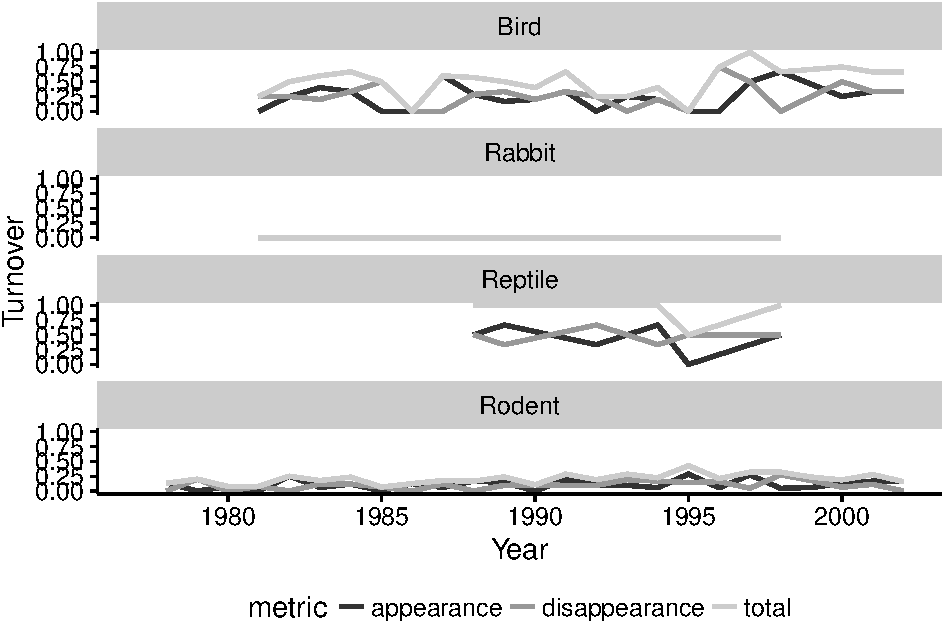
\includegraphics{temporal_assignment_files/figure-latex/unnamed-chunk-6-1.pdf}

\begin{Shaded}
\begin{Highlighting}[]
\CommentTok{# Low turnover is indicative of a stable community and high turnover is indicative of a dynamic community}
\end{Highlighting}
\end{Shaded}

\textbf{\emph{Question 5}}: a. How does temporal turnover relate to
spatial turnover? b. Which taxonomic group appears to be the most
variable? Which group appears to be the least variable?

\begin{quote}
\textbf{\emph{Answer 5a}}:Temporal turnover is a measure of change in
species composition over time for one location. Spatial turnover is a
measure of change in species composition between two locations for one
time point (i.e.~species gain or lost with cumulative area).
\end{quote}

\begin{quote}
\textbf{\emph{Answer 5b}}: Rodent communities are the least variable.
While, Bird and reptile communities tend to be more variable.
\end{quote}

\subsubsection{Mean Rank Shift}\label{mean-rank-shift}

In the code chunk below, do the following:

\begin{enumerate}
\def\labelenumi{\arabic{enumi}.}
\tightlist
\item
  Choose two plot\_types or two plot\_ids and compare the mean rank
  shift (MRS) between them.
\item
  Plot MRS for each through time.
\end{enumerate}

\begin{Shaded}
\begin{Highlighting}[]
\CommentTok{# Pull out the two treatments we analyzed earlier}
\NormalTok{portal.species.abunds =}\StringTok{ }\NormalTok{portal %>%}\StringTok{ }
\StringTok{                        }\KeywordTok{group_by}\NormalTok{(year, plot_type) %>%}\StringTok{ }
\StringTok{                        }\KeywordTok{count}\NormalTok{(taxon)}

\NormalTok{portal.abunds.cont.rodent =}\StringTok{ }\KeywordTok{filter}\NormalTok{(portal.species.abunds,}
\NormalTok{plot_type ==}\StringTok{ "Control"} \NormalTok{|}\StringTok{ }\NormalTok{plot_type ==}\StringTok{ "Rodent Exclosure"}\NormalTok{)}

\CommentTok{# Calculate MRS}
\NormalTok{portal.rankshift =}\StringTok{ }\KeywordTok{rank_shift}\NormalTok{(}\DataTypeTok{df =} \KeywordTok{as.data.frame}\NormalTok{(portal.abunds.cont.rodent), }
                              \DataTypeTok{time.var =} \StringTok{"year"}\NormalTok{,}
                              \DataTypeTok{species.var =} \StringTok{"taxon"}\NormalTok{,}
                              \DataTypeTok{abundance.var =} \StringTok{"n"}\NormalTok{,}
                              \DataTypeTok{replicate.var =} \StringTok{"plot_type"}\NormalTok{)}

\CommentTok{# Replace the year range with a single value to plot}
\NormalTok{portal.rankshift$year =}\StringTok{ }\KeywordTok{as.numeric}\NormalTok{(}\KeywordTok{substr}\NormalTok{(portal.rankshift$year_pair, }\DecValTok{6}\NormalTok{, }\DecValTok{9}\NormalTok{))}

\CommentTok{# Create ggplot}
\NormalTok{rankshift.plot =}\StringTok{  }\KeywordTok{ggplot}\NormalTok{(portal.rankshift, }\KeywordTok{aes}\NormalTok{(}\DataTypeTok{x =} \NormalTok{year, }\DataTypeTok{y =} \NormalTok{MRS, }\DataTypeTok{color =} \NormalTok{plot_type)) +}\StringTok{ }\KeywordTok{geom_line}\NormalTok{(}\DataTypeTok{size =} \DecValTok{1}\NormalTok{) +}
\KeywordTok{xlim}\NormalTok{(}\DecValTok{1977}\NormalTok{, }\DecValTok{2002}\NormalTok{) +}
\KeywordTok{xlab}\NormalTok{(}\StringTok{"Year"}\NormalTok{) +}
\KeywordTok{ylab}\NormalTok{(}\StringTok{"Mean Rank Shift"}\NormalTok{) +}\StringTok{ }\KeywordTok{scale_color_grey}\NormalTok{()}
\KeywordTok{plot}\NormalTok{(rankshift.plot)}
\end{Highlighting}
\end{Shaded}

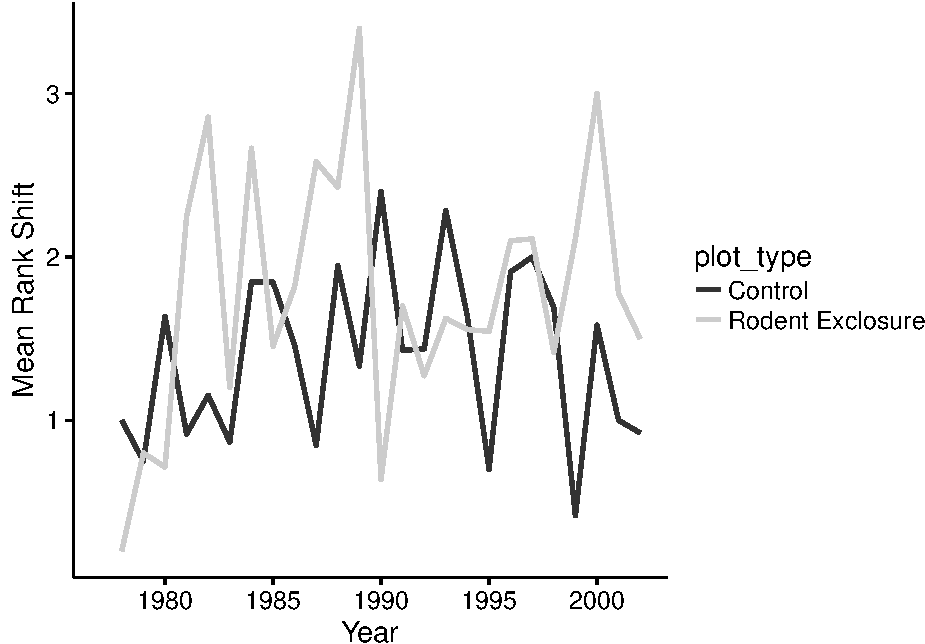
\includegraphics{temporal_assignment_files/figure-latex/unnamed-chunk-7-1.pdf}

\begin{Shaded}
\begin{Highlighting}[]
\NormalTok{portal.rankshift %>%}\StringTok{ }
\StringTok{  }\KeywordTok{group_by} \NormalTok{(plot_type) %>%}\StringTok{ }
\StringTok{  }\KeywordTok{summarise}\NormalTok{(}\DataTypeTok{mean =} \KeywordTok{mean}\NormalTok{(MRS), }\DataTypeTok{cv =} \KeywordTok{sd}\NormalTok{(MRS)/mean)}
\end{Highlighting}
\end{Shaded}

\begin{verbatim}
## # A tibble: 2 × 3
##          plot_type     mean        cv
##              <chr>    <dbl>     <dbl>
## 1          Control 1.400675 0.3759483
## 2 Rodent Exclosure 1.788980 0.4361809
\end{verbatim}

\textbf{\emph{Question 6}}:

\begin{enumerate}
\def\labelenumi{\alph{enumi}.}
\tightlist
\item
  What does a change in the rank shift tell you about the community?
\item
  Interpret the analysis and figure you just made.
\end{enumerate}

\begin{quote}
\textbf{\emph{Answer 6a}}: The change in the rank shift tells you
whether there are changes in commonness or rarity of taxa. The higher
the MRS index the greater the change.
\end{quote}

\begin{quote}
\textbf{\emph{Answer 6b}}: The plot shows higher MRS values for Rodent
exclosures on average. However, the MRS values are also more variable
for the rodent exclosures (CV = 0.44 compared to a CV = 0.38 for the
control plots).
\end{quote}

\subsubsection{Rate Change Interval}\label{rate-change-interval}

In the R code chunk below, do the following:

\begin{enumerate}
\def\labelenumi{\arabic{enumi}.}
\tightlist
\item
  Calculate the rate change interval using the Hellinger distance.
\item
  Plot the results.
\end{enumerate}

\begin{Shaded}
\begin{Highlighting}[]
\CommentTok{# In order to calculate relative abundances, we need total abundances # Let's add a column for total abundances}
\CommentTok{# We will relativize species abundances across the whole dataset so}
\CommentTok{# the transformed distances are preserved }
\NormalTok{portal.species.abunds$tot.abund =}\StringTok{ }\KeywordTok{rep}\NormalTok{(}\KeywordTok{sum}\NormalTok{(portal.species.abunds$n),}
\KeywordTok{length}\NormalTok{(portal.species.abunds$n))}

\CommentTok{# Now Apply the Hellinger transformation}
\NormalTok{portal.hellinger.transf =}\StringTok{ }\NormalTok{portal.species.abunds %>%}
\KeywordTok{mutate}\NormalTok{(}\DataTypeTok{hellinger.transf =} \KeywordTok{sqrt}\NormalTok{(n /}\StringTok{ }\NormalTok{tot.abund))}

\CommentTok{# The mutate function creates a new column "hellinger.transf"}
\CommentTok{# by taking the square root of species relative abundance}
\CommentTok{# We can use this new column as our "abundance" vector}
\NormalTok{portal.change.int =}\StringTok{ }\KeywordTok{rate_change_interval}\NormalTok{(portal.hellinger.transf, }\DataTypeTok{time.var =} \StringTok{"year"}\NormalTok{,}
                     \DataTypeTok{species.var =} \StringTok{"taxon"}\NormalTok{,}
                     \DataTypeTok{abundance.var =} \StringTok{"hellinger.transf"}\NormalTok{,}
                     \DataTypeTok{replicate.var =} \StringTok{"plot_type"}\NormalTok{)}

\NormalTok{rate.plot =}\StringTok{ }\KeywordTok{ggplot}\NormalTok{(portal.change.int, }\KeywordTok{aes}\NormalTok{(interval, distance)) +}
\StringTok{            }\KeywordTok{geom_point}\NormalTok{() +}
\StringTok{            }\KeywordTok{facet_wrap}\NormalTok{(~plot_type) +}\StringTok{ }
\StringTok{            }\KeywordTok{theme}\NormalTok{(}\DataTypeTok{strip.text.x =} \KeywordTok{element_text}\NormalTok{(}\DataTypeTok{size =} \DecValTok{7}\NormalTok{)) +}
\StringTok{            }\KeywordTok{stat_smooth}\NormalTok{(}\DataTypeTok{method =} \StringTok{"loess"}\NormalTok{, }\DataTypeTok{se =} \NormalTok{F, }\DataTypeTok{size =} \DecValTok{1}\NormalTok{) +}\StringTok{ }
\StringTok{            }\KeywordTok{ylab}\NormalTok{(}\StringTok{"Hellinger Distance"}\NormalTok{) +}
\StringTok{            }\KeywordTok{xlab}\NormalTok{(}\StringTok{"Time Interval (Years)"}\NormalTok{)}
\NormalTok{rate.plot}
\end{Highlighting}
\end{Shaded}

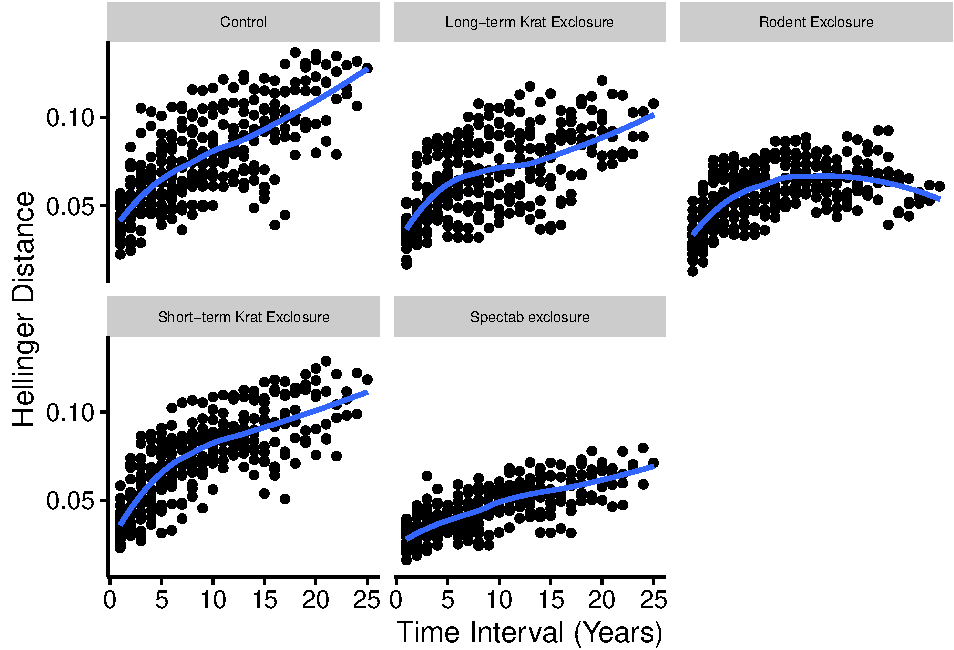
\includegraphics{temporal_assignment_files/figure-latex/unnamed-chunk-8-1.pdf}

\textbf{\emph{Question 7}}:

\begin{enumerate}
\def\labelenumi{\alph{enumi}.}
\tightlist
\item
  What does it mean to calculate a distance metric across varying time
  intervals?
\item
  Interpret the overall results. Develop a hypothesis based on the
  different responses of each treatment.
\end{enumerate}

\begin{quote}
\textbf{\emph{Answer 7a}}: You are calculating a rate change interval-
from which- you can tell how much a community is diverging over time and
the rate at which the divergence is happening.
\end{quote}

\begin{quote}
\textbf{\emph{Answer 7b}}: Hellinger distances tend to increase over
time for all of the exclosures except for the rodent exclosures. This
decrease in abundance in rodent exclosures may be due to a change in
competition dynamics. In the Rodent-Exclosure plots seed-eating desert
rodents were excluded. H: Interspecific competition for seeds increased
among smaller species in the Rodent Exclosure plots, resulting in
decreased abundances over time.
\end{quote}

\subsection{7) STABILITY}\label{stability}

In the R code chunk below, do the following:

\begin{enumerate}
\def\labelenumi{\arabic{enumi}.}
\tightlist
\item
  Using total abundance as your focal variable, calculate stability
  (i.e., 1/CV) and synchrony for each plot type.
\item
  Test for a biodiversity-stability relationship by regressing community
  stability on mean richness.
\item
  Test for a biodiversity-stability relationship by regressing community
  stability on mean inverse Simpson's diversity.
\end{enumerate}

\begin{Shaded}
\begin{Highlighting}[]
\CommentTok{# 1. Using total abundance as your focal variable, calculate stability (i.e., 1/CV) and synchrony for each plot type.}
\NormalTok{portal.stab =}\StringTok{ }\KeywordTok{community_stability}\NormalTok{(}\DataTypeTok{df =} \KeywordTok{as.data.frame}\NormalTok{(portal.species.abunds), }\DataTypeTok{time.var =} \StringTok{"year"}\NormalTok{,}
\DataTypeTok{abundance.var =} \StringTok{"n"}\NormalTok{,}\DataTypeTok{replicate.var =} \StringTok{"plot_type"}\NormalTok{)}
\KeywordTok{pander}\NormalTok{(portal.stab)}
\end{Highlighting}
\end{Shaded}

\begin{longtable}[c]{@{}cc@{}}
\toprule
\begin{minipage}[b]{0.34\columnwidth}\centering\strut
plot\_type
\strut\end{minipage} &
\begin{minipage}[b]{0.14\columnwidth}\centering\strut
stability
\strut\end{minipage}\tabularnewline
\midrule
\endhead
\begin{minipage}[t]{0.34\columnwidth}\centering\strut
Control
\strut\end{minipage} &
\begin{minipage}[t]{0.14\columnwidth}\centering\strut
3.044
\strut\end{minipage}\tabularnewline
\begin{minipage}[t]{0.34\columnwidth}\centering\strut
Long-term Krat Exclosure
\strut\end{minipage} &
\begin{minipage}[t]{0.14\columnwidth}\centering\strut
1.865
\strut\end{minipage}\tabularnewline
\begin{minipage}[t]{0.34\columnwidth}\centering\strut
Rodent Exclosure
\strut\end{minipage} &
\begin{minipage}[t]{0.14\columnwidth}\centering\strut
1.864
\strut\end{minipage}\tabularnewline
\begin{minipage}[t]{0.34\columnwidth}\centering\strut
Short-term Krat Exclosure
\strut\end{minipage} &
\begin{minipage}[t]{0.14\columnwidth}\centering\strut
2.462
\strut\end{minipage}\tabularnewline
\begin{minipage}[t]{0.34\columnwidth}\centering\strut
Spectab exclosure
\strut\end{minipage} &
\begin{minipage}[t]{0.14\columnwidth}\centering\strut
2.911
\strut\end{minipage}\tabularnewline
\bottomrule
\end{longtable}

\begin{Shaded}
\begin{Highlighting}[]
\CommentTok{# Here, we will calculate two measures of community-wide synchrony that range from −1 for perfect asynchrony to +1 for perfect synchrony.}

\NormalTok{portal.loreau =}\StringTok{ }\KeywordTok{synchrony}\NormalTok{(}\DataTypeTok{df =} \KeywordTok{as.data.frame}\NormalTok{(portal.species.abunds), }\DataTypeTok{time.var =} \StringTok{"year"}\NormalTok{,}
                \DataTypeTok{species.var =} \StringTok{"taxon"}\NormalTok{,}
                \DataTypeTok{abundance.var =} \StringTok{"n"}\NormalTok{,}
                \DataTypeTok{replicate.var =} \StringTok{"plot_type"}\NormalTok{,}
                \DataTypeTok{metric =} \StringTok{"Loreau"}\NormalTok{)}
\KeywordTok{names}\NormalTok{(portal.loreau)[}\DecValTok{2}\NormalTok{] =}\StringTok{ "loreau"}

\NormalTok{portal.gross =}\StringTok{ }\KeywordTok{synchrony}\NormalTok{(}\DataTypeTok{df =} \KeywordTok{as.data.frame}\NormalTok{(portal.species.abunds), }\DataTypeTok{time.var =} \StringTok{"year"}\NormalTok{,}
               \DataTypeTok{species.var =} \StringTok{"taxon"}\NormalTok{,}
               \DataTypeTok{abundance.var =} \StringTok{"n"}\NormalTok{,}
               \DataTypeTok{replicate.var =} \StringTok{"plot_type"}\NormalTok{,}
               \DataTypeTok{metric =} \StringTok{"Gross"}\NormalTok{)}
\KeywordTok{names}\NormalTok{(portal.gross)[}\DecValTok{2}\NormalTok{] =}\StringTok{ "gross"}
\KeywordTok{pander}\NormalTok{(}\KeywordTok{full_join}\NormalTok{(portal.loreau, portal.gross))}
\end{Highlighting}
\end{Shaded}

\begin{verbatim}
## Joining, by = "plot_type"
\end{verbatim}

\begin{longtable}[c]{@{}ccc@{}}
\toprule
\begin{minipage}[b]{0.33\columnwidth}\centering\strut
plot\_type
\strut\end{minipage} &
\begin{minipage}[b]{0.11\columnwidth}\centering\strut
loreau
\strut\end{minipage} &
\begin{minipage}[b]{0.11\columnwidth}\centering\strut
gross
\strut\end{minipage}\tabularnewline
\midrule
\endhead
\begin{minipage}[t]{0.33\columnwidth}\centering\strut
Control
\strut\end{minipage} &
\begin{minipage}[t]{0.11\columnwidth}\centering\strut
0.1869
\strut\end{minipage} &
\begin{minipage}[t]{0.11\columnwidth}\centering\strut
0.1263
\strut\end{minipage}\tabularnewline
\begin{minipage}[t]{0.33\columnwidth}\centering\strut
Long-term Krat Exclosure
\strut\end{minipage} &
\begin{minipage}[t]{0.11\columnwidth}\centering\strut
0.1578
\strut\end{minipage} &
\begin{minipage}[t]{0.11\columnwidth}\centering\strut
0.07418
\strut\end{minipage}\tabularnewline
\begin{minipage}[t]{0.33\columnwidth}\centering\strut
Rodent Exclosure
\strut\end{minipage} &
\begin{minipage}[t]{0.11\columnwidth}\centering\strut
0.187
\strut\end{minipage} &
\begin{minipage}[t]{0.11\columnwidth}\centering\strut
0.1423
\strut\end{minipage}\tabularnewline
\begin{minipage}[t]{0.33\columnwidth}\centering\strut
Short-term Krat Exclosure
\strut\end{minipage} &
\begin{minipage}[t]{0.11\columnwidth}\centering\strut
0.08773
\strut\end{minipage} &
\begin{minipage}[t]{0.11\columnwidth}\centering\strut
0.001546
\strut\end{minipage}\tabularnewline
\begin{minipage}[t]{0.33\columnwidth}\centering\strut
Spectab exclosure
\strut\end{minipage} &
\begin{minipage}[t]{0.11\columnwidth}\centering\strut
0.1542
\strut\end{minipage} &
\begin{minipage}[t]{0.11\columnwidth}\centering\strut
0.1393
\strut\end{minipage}\tabularnewline
\bottomrule
\end{longtable}

\begin{Shaded}
\begin{Highlighting}[]
\CommentTok{# 2. Test for a biodiversity-stability relationship by regressing community stability on mean richness.}
\CommentTok{# Recall, earlier we calculated richness in each plot type in each year # Let's group only by plot_id}
\CommentTok{# Then, we we summarise average annual richness in each plot type}
\NormalTok{richness =}\StringTok{ }\KeywordTok{as.data.frame}\NormalTok{(}\KeywordTok{rowSums}\NormalTok{(time.by.species[,-}\KeywordTok{c}\NormalTok{(}\DecValTok{1}\NormalTok{:}\DecValTok{3}\NormalTok{)]>}\DecValTok{0}\NormalTok{))}
\NormalTok{rich.all =}\StringTok{ }\KeywordTok{data.frame}\NormalTok{(time.by.species[,}\DecValTok{1}\NormalTok{:}\DecValTok{3}\NormalTok{,], richness)}
\KeywordTok{names}\NormalTok{(rich.all)[}\DecValTok{4}\NormalTok{] =}\StringTok{ "richness"}
\NormalTok{rich.treat =}\StringTok{ }\NormalTok{rich.all[}\KeywordTok{which}\NormalTok{(rich.all$plot_type ==}\StringTok{ "Control"}\NormalTok{|}\StringTok{ }\NormalTok{rich.all$plot_type ==}\StringTok{ "Rodent Exclosure"}\NormalTok{), ]}
\NormalTok{portal.mean.rich.plot =}\StringTok{ }\NormalTok{rich.all %>%}
\StringTok{                        }\KeywordTok{group_by}\NormalTok{(plot_id) %>%}\StringTok{ }
\StringTok{                        }\KeywordTok{summarise}\NormalTok{(}\DataTypeTok{mean.rich =} \KeywordTok{mean}\NormalTok{(richness))}
\CommentTok{# Let's take a look at how stability metrics relate to mean richness}
\NormalTok{portal.plot.abunds =}\StringTok{ }\KeywordTok{as.data.frame}\NormalTok{( }\KeywordTok{group_by}\NormalTok{(portal, year, plot_id) %>%}\StringTok{ }\KeywordTok{count}\NormalTok{(taxon))}
\NormalTok{portal.stab.plot =}\StringTok{ }\KeywordTok{community_stability}\NormalTok{(}\DataTypeTok{df =} \NormalTok{portal.plot.abunds, }\DataTypeTok{time.var =} \StringTok{"year"}\NormalTok{,}
                    \DataTypeTok{abundance.var =} \StringTok{"n"}\NormalTok{, }\DataTypeTok{replicate.var =} \StringTok{"plot_id"}\NormalTok{)}
\CommentTok{# Join richness and stability}
\NormalTok{portal.div.stab =}\StringTok{ }\NormalTok{portal.mean.rich.plot %>%}
\StringTok{                  }\KeywordTok{inner_join}\NormalTok{(portal.stab.plot)}
\end{Highlighting}
\end{Shaded}

\begin{verbatim}
## Joining, by = "plot_id"
\end{verbatim}

\begin{Shaded}
\begin{Highlighting}[]
\CommentTok{# Plot the relationship}
\KeywordTok{par}\NormalTok{(}\DataTypeTok{mar =} \KeywordTok{c}\NormalTok{(}\DecValTok{5}\NormalTok{,}\DecValTok{5}\NormalTok{,}\DecValTok{1}\NormalTok{,}\DecValTok{1}\NormalTok{))}
\KeywordTok{plot}\NormalTok{(portal.div.stab$stability ~}\StringTok{ }\NormalTok{portal.div.stab$mean.rich,}
     \DataTypeTok{xlab =} \StringTok{"Mean Richness"}\NormalTok{, }\DataTypeTok{ylab =} \StringTok{"Average Stability"}\NormalTok{, }\DataTypeTok{yaxt =} \StringTok{"n"}\NormalTok{, }\DataTypeTok{xaxt =} \StringTok{"n"}\NormalTok{,}
\DataTypeTok{xlim =} \KeywordTok{c}\NormalTok{(}\DecValTok{2}\NormalTok{,}\DecValTok{10}\NormalTok{), }\DataTypeTok{ylim =} \KeywordTok{c}\NormalTok{(}\DecValTok{1}\NormalTok{,}\DecValTok{4}\NormalTok{))}
\KeywordTok{axis}\NormalTok{(}\DataTypeTok{side =} \DecValTok{1}\NormalTok{, }\DataTypeTok{cex.axis =} \FloatTok{1.2}\NormalTok{, }\DataTypeTok{lwd.ticks =} \DecValTok{2}\NormalTok{, }\DataTypeTok{las =} \DecValTok{1}\NormalTok{) }
\KeywordTok{axis}\NormalTok{(}\DataTypeTok{side =} \DecValTok{2}\NormalTok{, }\DataTypeTok{cex.axis =} \FloatTok{1.2}\NormalTok{, }\DataTypeTok{lwd.ticks =} \DecValTok{2}\NormalTok{, }\DataTypeTok{las =} \DecValTok{1}\NormalTok{) }
\KeywordTok{axis}\NormalTok{(}\DataTypeTok{side =} \DecValTok{3}\NormalTok{, }\DataTypeTok{lwd.ticks =} \DecValTok{2}\NormalTok{, }\DataTypeTok{las =} \DecValTok{1}\NormalTok{, }\DataTypeTok{labels =} \NormalTok{F)}
\KeywordTok{axis}\NormalTok{(}\DataTypeTok{side =} \DecValTok{4}\NormalTok{, }\DataTypeTok{lwd.ticks =} \DecValTok{2}\NormalTok{, }\DataTypeTok{las =} \DecValTok{1}\NormalTok{, }\DataTypeTok{labels =} \NormalTok{F)}
\KeywordTok{box}\NormalTok{(}\DataTypeTok{lwd =} \DecValTok{2}\NormalTok{)}
\NormalTok{div.stab.lm =}\StringTok{ }\KeywordTok{lm}\NormalTok{(portal.div.stab$stability ~}\StringTok{ }\NormalTok{portal.div.stab$mean.rich) }
\KeywordTok{abline}\NormalTok{(div.stab.lm)}
\NormalTok{r2 =}\StringTok{ }\KeywordTok{bquote}\NormalTok{(}\KeywordTok{italic}\NormalTok{(R)^}\DecValTok{2} \NormalTok{==}\StringTok{ }\NormalTok{.(}\KeywordTok{format}\NormalTok{(}\KeywordTok{summary}\NormalTok{(div.stab.lm)$adj.r.square, }\DataTypeTok{digits =} \DecValTok{3}\NormalTok{)))}
\KeywordTok{text}\NormalTok{(}\FloatTok{3.25}\NormalTok{,}\FloatTok{3.75}\NormalTok{, }\DataTypeTok{cex =} \FloatTok{1.5}\NormalTok{, }\DataTypeTok{labels =} \NormalTok{r2)}
\end{Highlighting}
\end{Shaded}

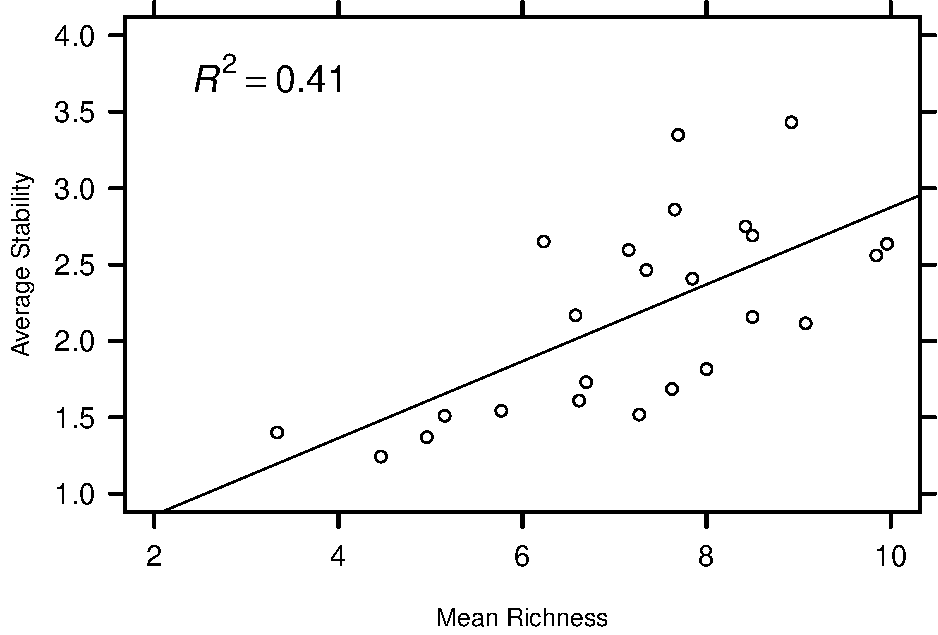
\includegraphics{temporal_assignment_files/figure-latex/unnamed-chunk-9-1.pdf}

\begin{Shaded}
\begin{Highlighting}[]
\CommentTok{# 3. Test for a biodiversity-stability relationship by regressing community stability on mean inverse Simpson's diversity.}

\CommentTok{# Recall, earlier we calculated 1/D in each plot type in each year }
\CommentTok{# Let's group only by plot_id}
\CommentTok{# Then, we we summarise average annual richness in each plot type }
\NormalTok{portal.mean.div.plot =}\StringTok{ }\NormalTok{div.all %>%}
\StringTok{                        }\KeywordTok{group_by}\NormalTok{(plot_id) %>%}\StringTok{ }
\StringTok{                        }\KeywordTok{summarise}\NormalTok{(}\DataTypeTok{mean.div =} \KeywordTok{mean}\NormalTok{(inv.simp))}
\CommentTok{# Let's take a look at how stability metrics relate to mean 1/D}
\NormalTok{portal.plot.abunds =}\StringTok{ }\KeywordTok{as.data.frame}\NormalTok{( }\KeywordTok{group_by}\NormalTok{(portal, year, plot_id) %>%}\StringTok{ }\KeywordTok{count}\NormalTok{(taxon))}
\NormalTok{portal.stab.plot.D =}\StringTok{ }\KeywordTok{community_stability}\NormalTok{(}\DataTypeTok{df =} \NormalTok{portal.plot.abunds, }\DataTypeTok{time.var =} \StringTok{"year"}\NormalTok{,}\DataTypeTok{abundance.var =} \StringTok{"n"}\NormalTok{, }\DataTypeTok{replicate.var =} \StringTok{"plot_id"}\NormalTok{)}
\CommentTok{# Join richness and stability}
\NormalTok{portal.div.stab.D =}\StringTok{ }\NormalTok{portal.mean.div.plot %>%}
\StringTok{                  }\KeywordTok{inner_join}\NormalTok{(portal.stab.plot.D)}
\end{Highlighting}
\end{Shaded}

\begin{verbatim}
## Joining, by = "plot_id"
\end{verbatim}

\begin{Shaded}
\begin{Highlighting}[]
\CommentTok{# Plot the relationship}
\KeywordTok{par}\NormalTok{(}\DataTypeTok{mar =} \KeywordTok{c}\NormalTok{(}\DecValTok{5}\NormalTok{,}\DecValTok{5}\NormalTok{,}\DecValTok{1}\NormalTok{,}\DecValTok{1}\NormalTok{))}
\KeywordTok{plot}\NormalTok{(portal.div.stab.D$stability ~}\StringTok{ }\NormalTok{portal.div.stab.D$mean.div,}
     \DataTypeTok{xlab =} \StringTok{"Mean Inverse Simpsons Diversity Index"}\NormalTok{, }\DataTypeTok{ylab =} \StringTok{"Aggregate Stability"}\NormalTok{, }\DataTypeTok{yaxt =} \StringTok{"n"}\NormalTok{, }\DataTypeTok{xaxt =} \StringTok{"n"}\NormalTok{,}
\DataTypeTok{xlim =} \KeywordTok{c}\NormalTok{(}\DecValTok{2}\NormalTok{,}\DecValTok{6}\NormalTok{), }\DataTypeTok{ylim =} \KeywordTok{c}\NormalTok{(}\DecValTok{1}\NormalTok{,}\DecValTok{4}\NormalTok{))}
\KeywordTok{axis}\NormalTok{(}\DataTypeTok{side =} \DecValTok{1}\NormalTok{, }\DataTypeTok{cex.axis =} \FloatTok{1.2}\NormalTok{, }\DataTypeTok{lwd.ticks =} \DecValTok{2}\NormalTok{, }\DataTypeTok{las =} \DecValTok{1}\NormalTok{) }
\KeywordTok{axis}\NormalTok{(}\DataTypeTok{side =} \DecValTok{2}\NormalTok{, }\DataTypeTok{cex.axis =} \FloatTok{1.2}\NormalTok{, }\DataTypeTok{lwd.ticks =} \DecValTok{2}\NormalTok{, }\DataTypeTok{las =} \DecValTok{1}\NormalTok{) }
\KeywordTok{axis}\NormalTok{(}\DataTypeTok{side =} \DecValTok{3}\NormalTok{, }\DataTypeTok{lwd.ticks =} \DecValTok{2}\NormalTok{, }\DataTypeTok{las =} \DecValTok{1}\NormalTok{, }\DataTypeTok{labels =} \NormalTok{F)}
\KeywordTok{axis}\NormalTok{(}\DataTypeTok{side =} \DecValTok{4}\NormalTok{, }\DataTypeTok{lwd.ticks =} \DecValTok{2}\NormalTok{, }\DataTypeTok{las =} \DecValTok{1}\NormalTok{, }\DataTypeTok{labels =} \NormalTok{F)}
\KeywordTok{box}\NormalTok{(}\DataTypeTok{lwd =} \DecValTok{2}\NormalTok{)}
\NormalTok{div.stab.lm.D =}\StringTok{ }\KeywordTok{lm}\NormalTok{(portal.div.stab.D$stability ~}\StringTok{ }\NormalTok{portal.div.stab.D$mean.div) }
\KeywordTok{abline}\NormalTok{(div.stab.lm.D)}
\NormalTok{r2 =}\StringTok{ }\KeywordTok{bquote}\NormalTok{(}\KeywordTok{italic}\NormalTok{(R)^}\DecValTok{2} \NormalTok{==}\StringTok{ }\NormalTok{.(}\KeywordTok{format}\NormalTok{(}\KeywordTok{summary}\NormalTok{(div.stab.lm.D)$adj.r.square, }\DataTypeTok{digits =} \DecValTok{3}\NormalTok{)))}
\KeywordTok{text}\NormalTok{(}\FloatTok{3.25}\NormalTok{,}\FloatTok{3.75}\NormalTok{, }\DataTypeTok{cex =} \FloatTok{1.5}\NormalTok{, }\DataTypeTok{labels =} \NormalTok{r2)}
\end{Highlighting}
\end{Shaded}

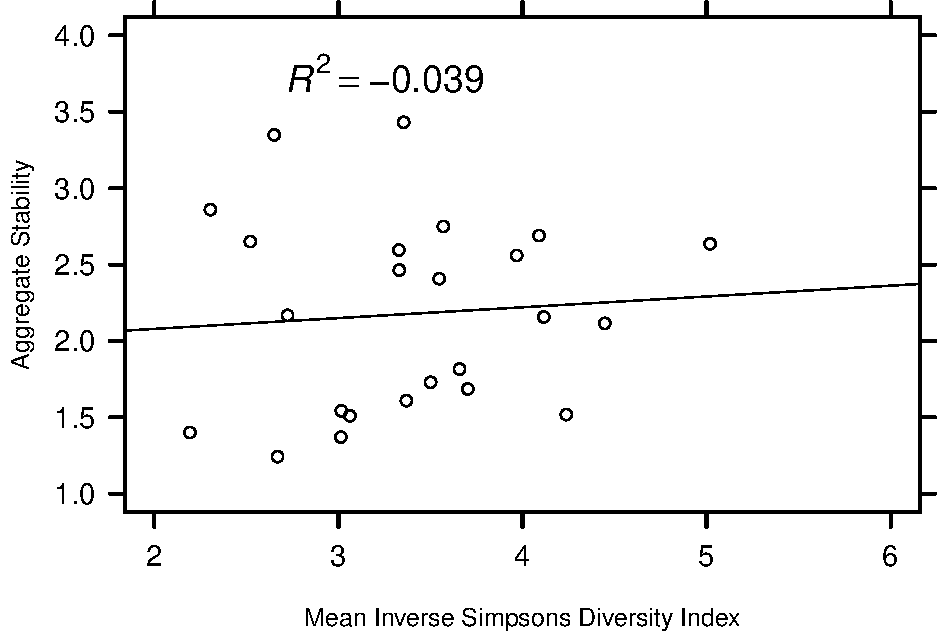
\includegraphics{temporal_assignment_files/figure-latex/unnamed-chunk-9-2.pdf}

\begin{Shaded}
\begin{Highlighting}[]
\KeywordTok{Sys.setenv}\NormalTok{(}\StringTok{"DISPLAY"}\NormalTok{=}\StringTok{":0"}\NormalTok{)}
\end{Highlighting}
\end{Shaded}

\textbf{\emph{Question 8}}:

\begin{enumerate}
\def\labelenumi{\alph{enumi}.}
\tightlist
\item
  Which plot type has the highest stability in total abundance? How is
  stability of total abundance measured with the function you learned?
  How does this measure of stability relate to the coefficient of
  variation?
\item
  In your own words, describe the concept of synchrony
\item
  Interpret the results from the biodiversity-stability relationships
  you analyzed.
\end{enumerate}

\begin{quote}
\textbf{\emph{Answer 8a}}: Control plots had the highest stability in
total abundance. The stability of total abundance is measured as the
inverse of the coefficient of variation (1/CV) and is equal to the mean
divided by the standard deviation. Higher CVs indicate lower stability
and lower CVs indicate greater stability.
\end{quote}

\begin{quote}
\textbf{\emph{Answer 8b}}: Synchrony is a measure of whether or not
population densities are in phase or in sync with one another, meaning
that they fluctuate in the same manner in response to a change in the
environment. When species display strong synchrony their densities
positively covary. \textbf{\emph{Answer 8c}}: Richness increases with
aggregate stability (total abundance; R2 = 0.41). However, mean inverse
Simpson's diversity slightly decreases with aggregate stability (R2 =
-0.039). It is generally thought that more diverse ecosystems are more
stable. The portal data do not seem to be consistent with this
expectation from biodiversity-stability theory.
\end{quote}

\subsection{SYNTHESIS}\label{synthesis}

Compare and contrast the core concepts from temporal and spatial
diversity (e.g., autocorrelation, scale, variability, etc.). Identify a
few of the major challenges associated with studying biodiversity
through time and across space.

\begin{quote}
\textbf{\emph{Synthesis}}:In order to analyze how biodiversity changes
across time and space, you must consider the possibility that some
samples in a dataset may not be independent - because samples taken
relatively close together in space or time are potentially redundant as
a result of autocorrelation. Accounting for repeated measurements on the
same variable is one of the challenges associated with comparing
diversity across time or space. Both spatial and temporal
autocorrelation can be detected through diagnostic plots. Variograms
show the distance at which you can compare diversity between sites. A
way of assessing temporal autocorrelation or the assumption of
stationarity, is to look at time lag plots using the ACF or PACF
function. Lags that are significantly correlated indicate that there may
be some temporal pattern to your data- for instance a lag at two,
indicated a seasonal signal (rainy vs.~dry season). If there is a
significant correlation at a lag, corrective measures should be taken
which involve transforming or differencing the data to get rid of the
trend. Both temporal and spatial analyses involve concepts of scale.
Spatial extent includes the entire area under investigation, whereas,
spatial grain is the smallest sampling unit (1 meter by 1 meter plots
for example). Temporal extent is the entire duration of the study (1
year) and temporal grain refers to the smallest observational unit
(minutes). Another challenge is defining the most appropriate scale
(grain and extent) for representing diversity in your system. There is
often a tradeoff in temporal and spatial resolution. Observations
collected at high temporal resolution (every hour) will often be limited
to a few locations. Whereas, studies that collect data at a high spatial
resolution- are usually only done at one point in time.
\end{quote}

\end{document}
